\section{Công trình liên quan}

\begin{frame}{Các phương pháp}
\textbf{Rule Base \& Statistic}
\begin{itemize}
	\small
	\item BEAT, Rule-based generation.
	%					 \cite{cassell2001beat}
	\item Gesture Controllers 
\end{itemize}
%	\textit{Nhược điểm}: Không có khả năng mở rộng, kết quả không tốt với các dữ liệu ngoài tập huấn luyện.

\textbf{Deep Learning}
%\begin{itemize}
%	\small
%	\item \textbf{MLP}: Gesticulator
%	\item \textbf{RNN}: Speech2AffectiveGestures, HA2G, TransGesture, .. 
%	\item \textbf{Normalising Flows}: Text2gestures, Speech2Gesture,; \textbf{GAN}: DiffGAN
%	\item \textbf{VAE/VQ-VAE}:  Audio2Gestures; 
%	\item \textbf{Diffusion}: Listen denoise action, DiffuseStyleGesture, Taming Diffusion Models.
%\end{itemize}
\begin{columns}
	\begin{column}{0.5\textwidth}
			{
			\small
			\textbf{Likelihood-based models}:
			\begin{itemize}
				\item \textbf{MLP}: Gesticulator
				\item \textbf{RNN}: Speech2AffectiveGestures, HA2G, TransGesture, .. 
				\item \textbf{Normalising Flows}: Text2gestures, Speech2Gesture
				\textbf{VAE/VQ-VAE}:  Audio2Gestures; 
				\end{itemize}
			}
			 \begin{figure}
				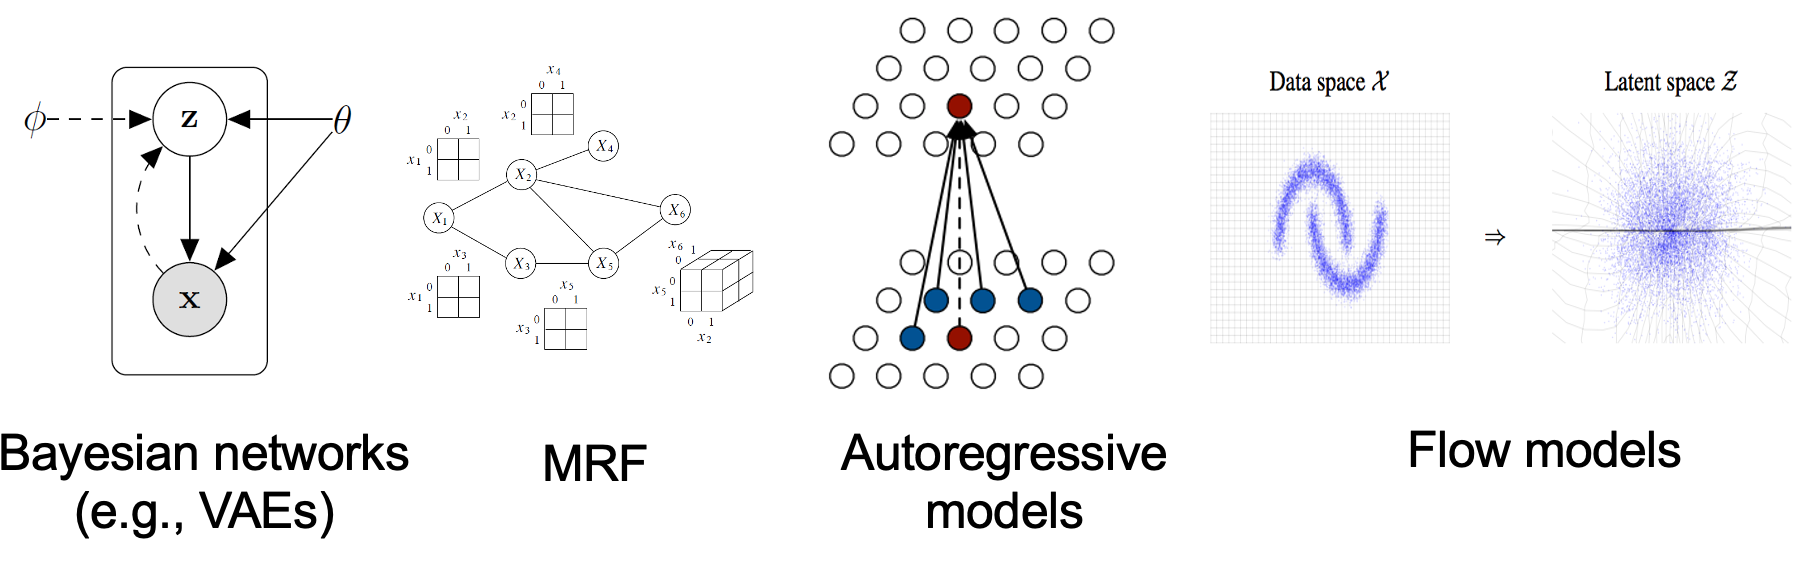
\includegraphics[width=\textwidth]{likelihood_based_models}
			\end{figure}
	\end{column}
	\hspace{-20pt}
	\begin{column}{0.5\textwidth}
		{
			\small
			\textbf{Implicit generative models}:
\begin{itemize}
			\item \textbf{GAN}: DiffGAN
			
			\item \textbf{Diffusion}: Listen denoise action, DiffuseStyleGesture, Taming Diffusion Models.
 \end{itemize}
 
 \begin{figure}
 	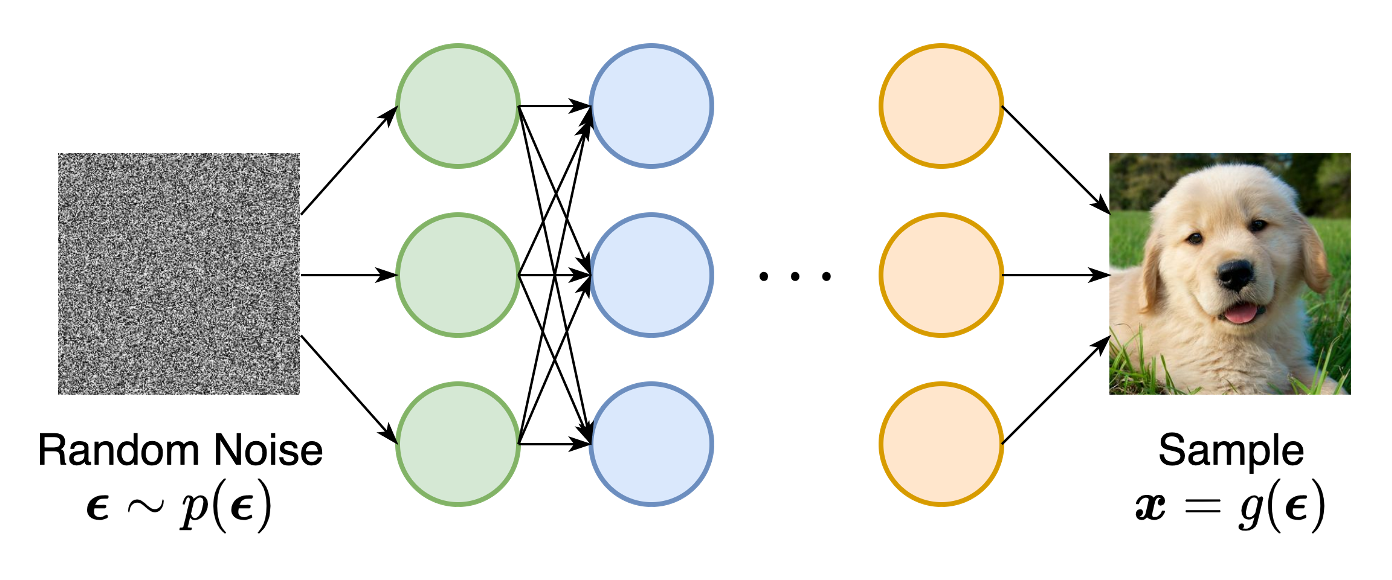
\includegraphics[width=\textwidth]{implicit_models}
 \end{figure}
 
		}
	\end{column}
\end{columns}

%	\textbf{Phase Manifold} : 
%	
%	\begin{itemize}
%		\small
%		\item  DeepPhase , Walk the Dog
%	\end{itemize}

	

%\textbf{Baseline}: \textit{Motion Diffusion Model} (MDM)

%\begin{columns}
%\begin{column}{0.55\textwidth}
	
%\end{column}			
% 
%	
%	\begin{column}{0.45\textwidth}
%		
%		\begin{columns}
%			\begin{column}{0.5\textwidth}
%				\begin{figure}
%					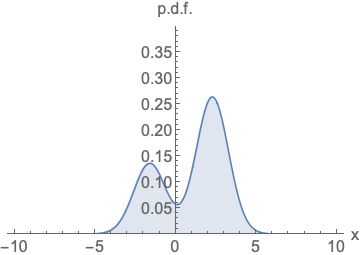
\includegraphics[width=\textwidth]{ProbabilityDensityFunctions.png}
%					\caption{\scriptsize Phải chuẩn hoá (diện tích dưới đường cong phải tích phân thành một)}
%				\end{figure}
%			\end{column}
%			\begin{column}{0.5\textwidth}
%				\begin{figure}
%					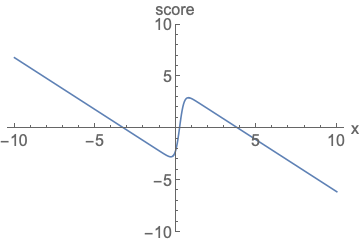
\includegraphics[width=\textwidth]{ScoreFunction.png}
%					\caption{\scriptsize Không cần chuẩn hoá.}
%				\end{figure}
%			\end{column}
%		\end{columns}
%	
%		\begin{columns}
%			\begin{column}{0.5\textwidth}
%				\centering
%				\begin{tikzpicture}
%					\node at (0, 1) {$p(\mathbf{x})$};
%					
%					\node at (0, 0.5) {\small \text{probability density}};
%					
%					\draw[<->, thick] (0, 0) -- (0, -0.5);
%					
%					\node at (0, -1) {$\nabla_\mathbf{x} \log p(\mathbf{x})$};
%					
%					\node at (0, -1.5) {\small \text{score function}};
%				\end{tikzpicture}
%				
%			\end{column}
%			\begin{column}{0.5\textwidth}
%				\begin{figure}
%					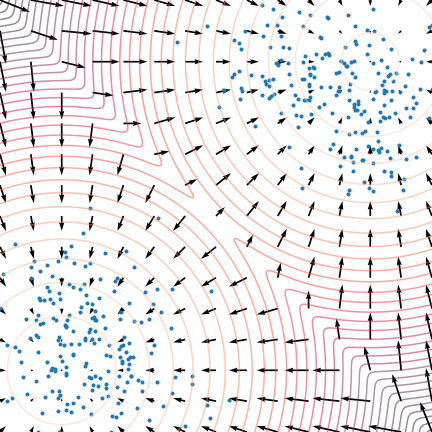
\includegraphics[width=\textwidth]{CompareScoreFunction.png}
%					\caption{\scriptsize score function vs probability density}
%				\end{figure}
%			\end{column}
%		\end{columns}
%	\end{column}
%\end{columns}

%\includegraphics[width=\linewidth]{../animation/ScoreFunction/ScoreFunction\_001}
	
\end{frame}



\begin{frame}{Tư tưởng cơ bản của Diffusion}
	Dataset $\mathcal{G} = \{ x_{i}^{M \times D} \}_{1}^{n}$, ta chuẩn hoá dữ liệu $\bx_{i}^{M \times D} = \frac{\bx_{i}^{M \times D} - \mu}{\sigma}$
\begin{figure}
	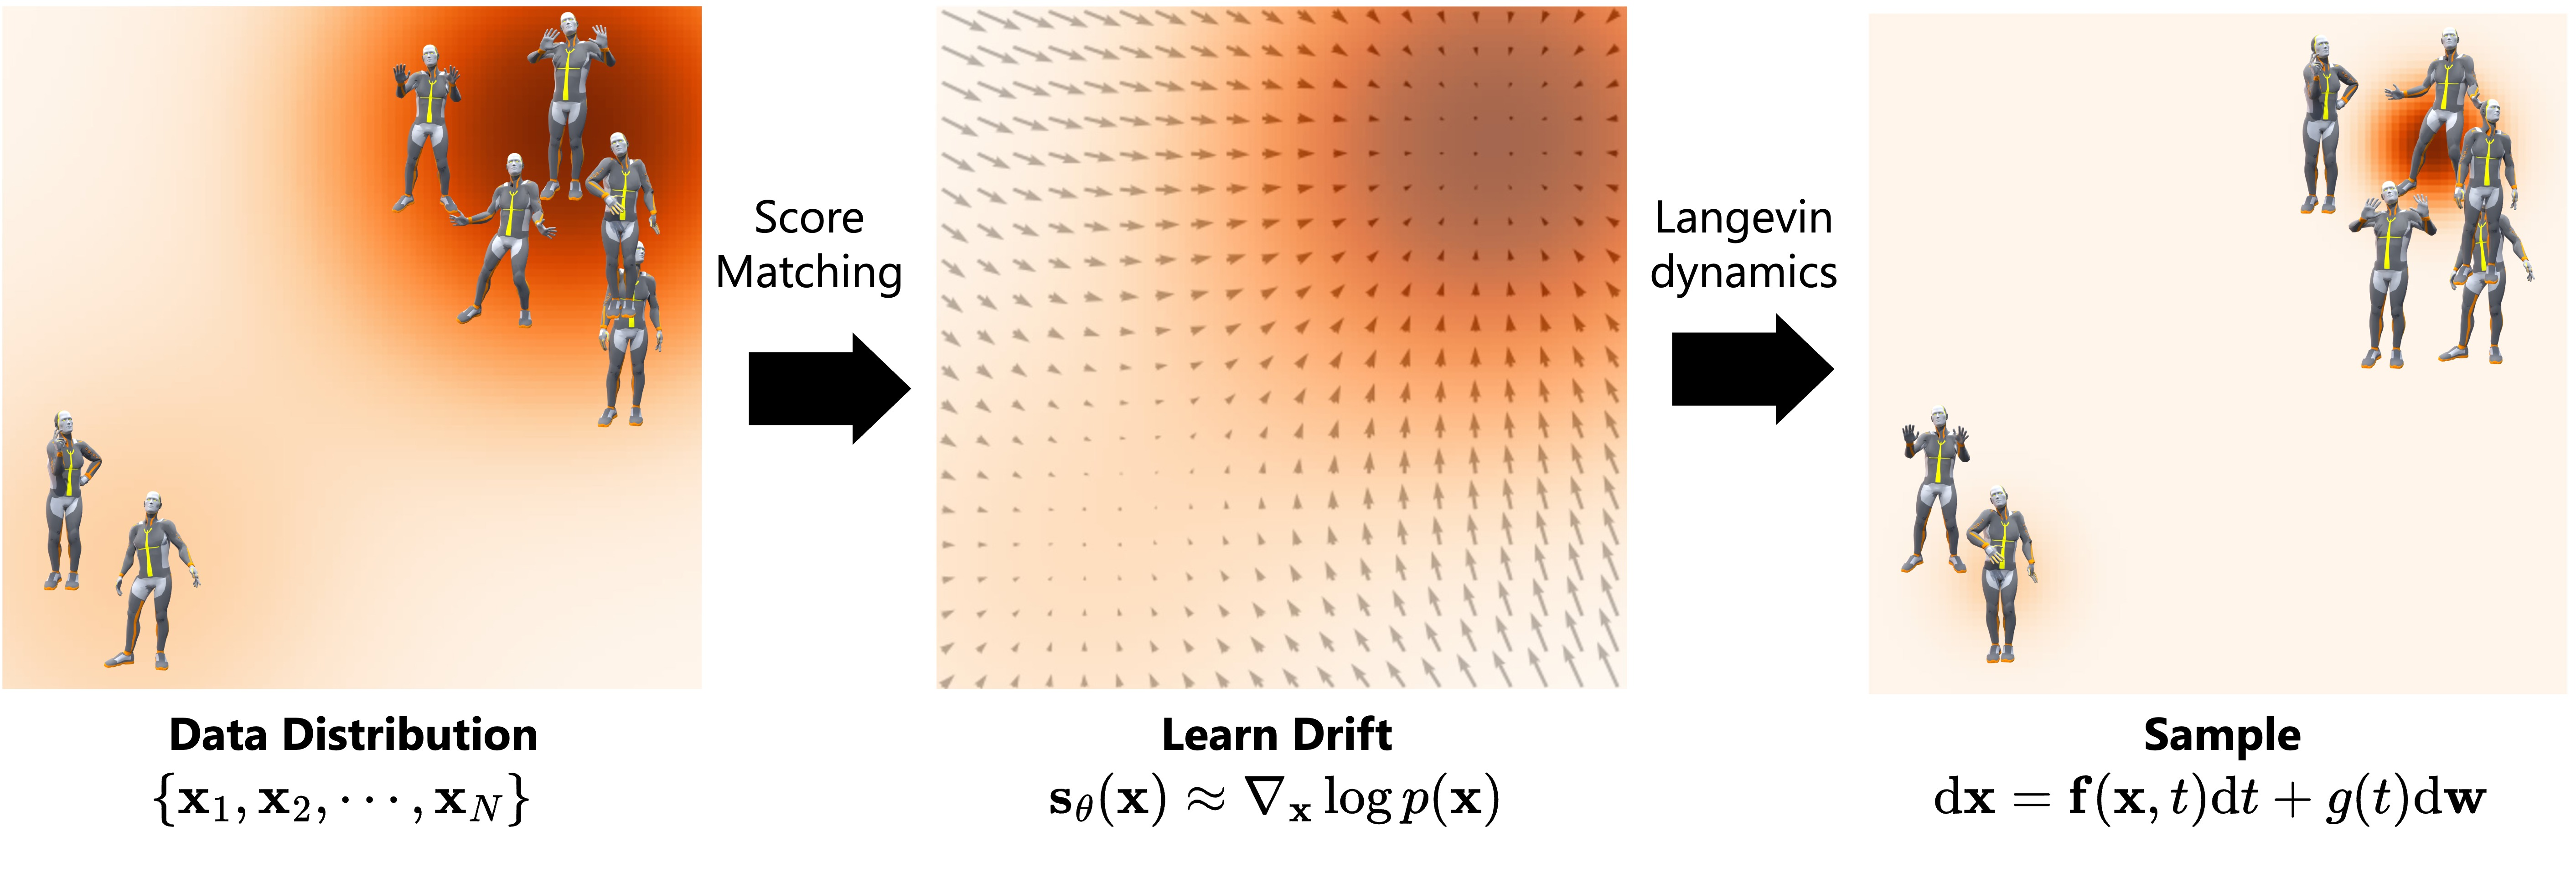
\includegraphics[width=0.8\textwidth]{ScoreMatching}
\end{figure}
\vspace{-10pt}
\begin{figure}
	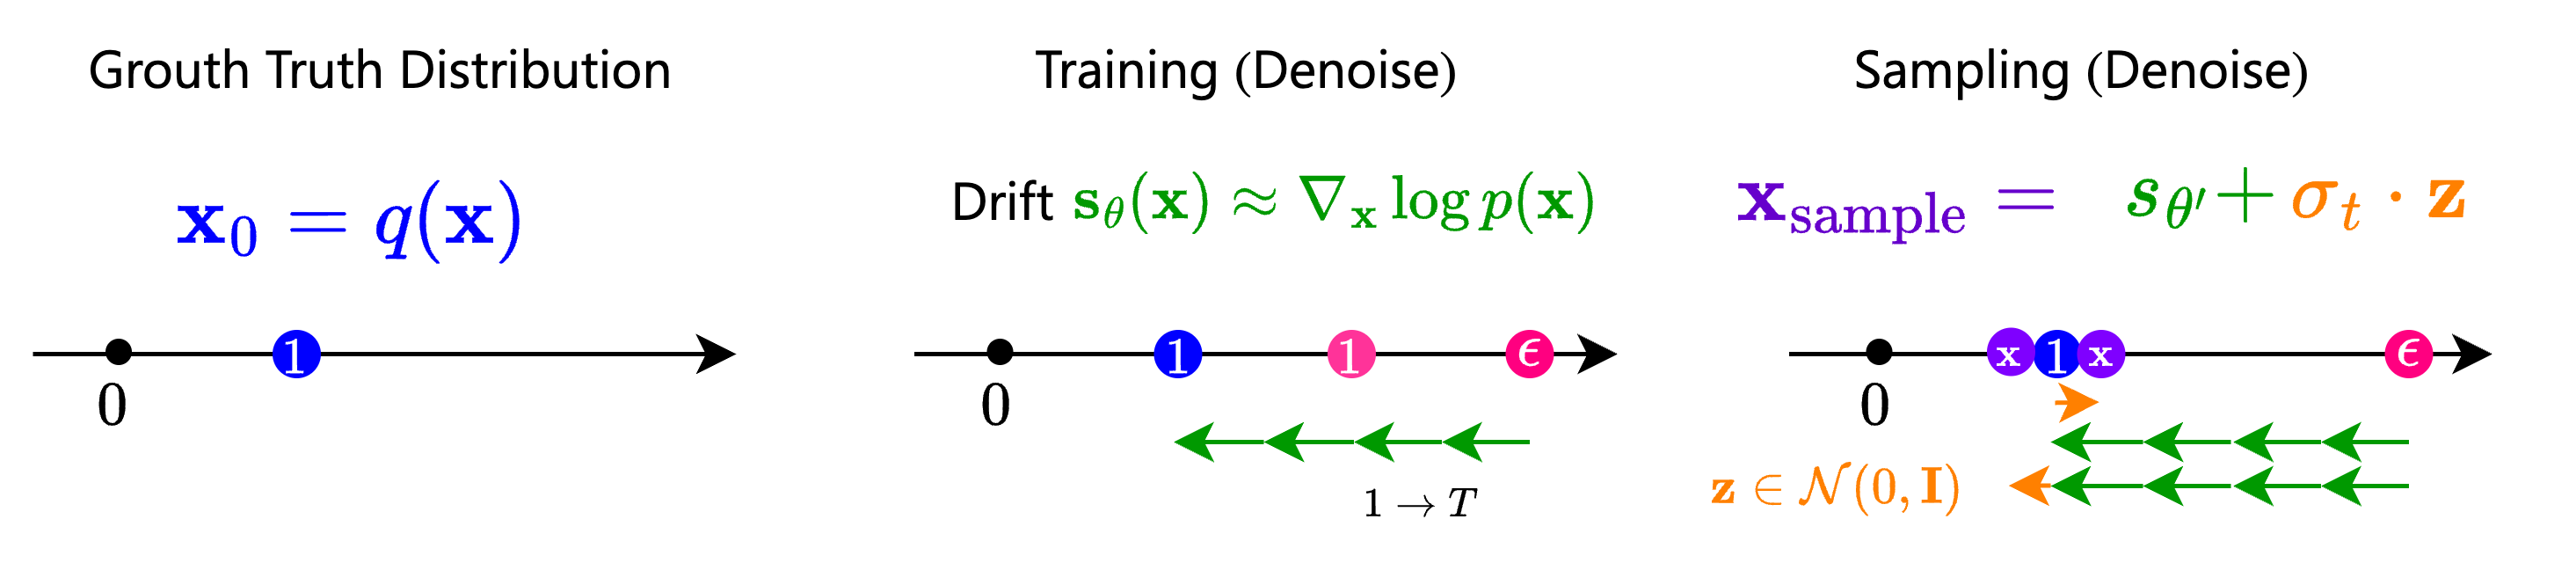
\includegraphics[width=\textwidth]{ScoreDrift}
\end{figure}

\vspace{-10pt}

\begin{figure}
	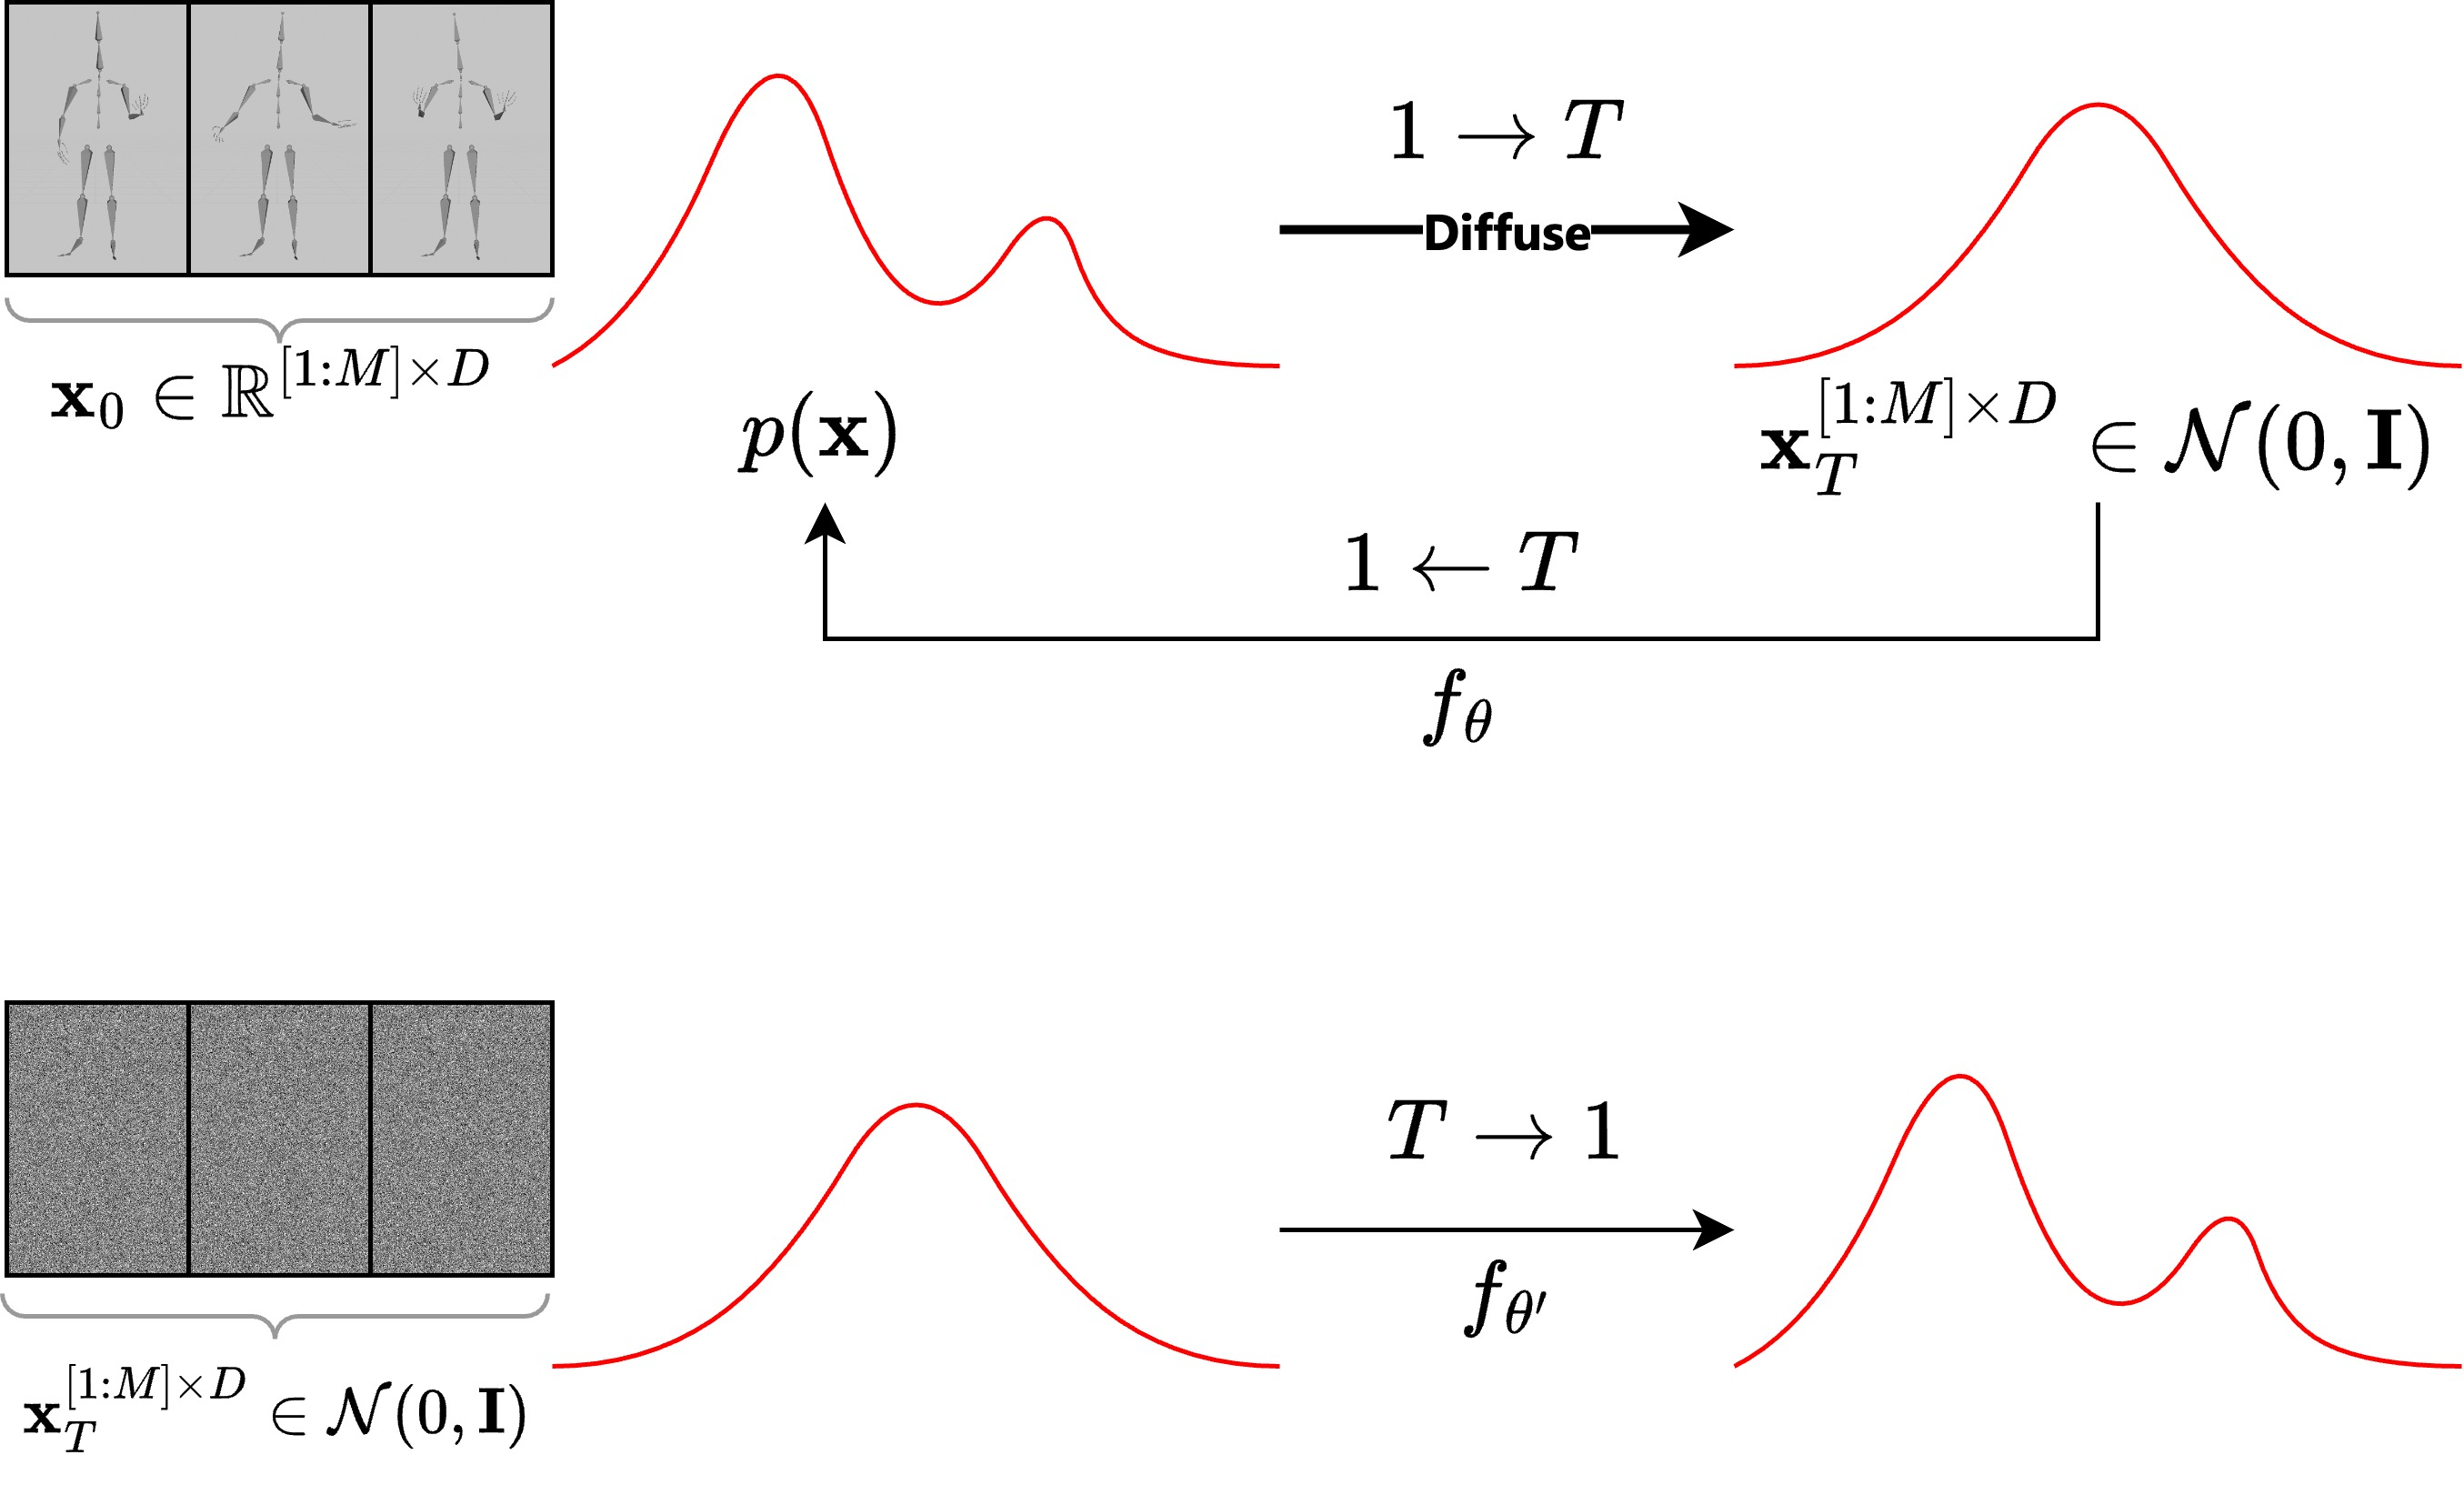
\includegraphics[width=0.8\textwidth]{DistributionTransition}
\end{figure}

\end{frame}

\begin{frame}{Ký hiệu}
	\textbf{Tham số}: Đang huấn luyện {\Large$\textcolor{cyan}{\theta}$}, đã huấn luyện xong: {\Large$\textcolor{cyan}{\theta}'$}, {\Large$\textcolor{cyan}{\hat{\bx}}$}: dự đoán
	\vspace{-5pt}
	
	\textbf{Phân phối chuẩn}
	\vspace{-5pt}
	{\Large $$\mathcal{N}(\textcolor{red}{a} \mathbf{x}, \textcolor{blue}{b^2})$$}
	\vspace{-15pt}
	\begin{itemize}
		\item Một hàm $f(x) = a x + b\epsilon$ với $\epsilon \in \mathcal{N}(0, \mathbf{1})$ được ký hiệu là $f(x) \sim \mathcal{N}(a x, b^2) $
		
		\item Trung bình: $\mu = \textcolor{red}{a}x=\frac{1}{n} \sum_{i=1}^{n} x_i$
		
		\item Phương sai: $\sigma^2 = \textcolor{blue} {b^2} = \frac{1}{n} \sum_{i=1}^{n} (x_i - \mu)^2$
		
	\end{itemize}
	\textbf{Xác xuất có điều kiện}
	\vspace{-5pt}
	{\Large $$p(\textcolor{green}{x}| \textcolor{orange}{y})$$}
	\vspace{-15pt}
	
	\begin{itemize}
		\item $p(\textcolor{green}{x}| \textcolor{orange}{y})$ là xác xuất có điều kiện.
		\item $\textcolor{orange}{y}$: xảy ra trước (bên phải)
		\item $\textcolor{green}{x}$: sảy ra sau y (bên trái)
	\end{itemize}

\end{frame}

\begin{frame}{Đặc điểm của việc học dữ liệu Motion}
	
	\begin{columns}
		\begin{column}{0.55\textwidth}
			\textbf{Quan hệ giữa dữ liệu cử chỉ và âm thanh}:
			\begin{itemize}
				\item Một đoạn cử có thể bao gồm nhiều âm thanh.
				\item Mỗi âm thanh có thể tương ứng với nhiều đoạn cử chỉ khác nhau.
			\end{itemize}
			%		Baseline: \textbf{MDM}  (Human Motion Diffusion Model)
			\textbf{Khó khăn}
			\begin{itemize}
				\item Dữ liệu ít, chi phí cao
				\item Thiếu nhãn và dữ liệu tương ứng giữa âm thanh, cử chỉ.
				\item Quá trình sinh có thể dể điều khiển 
				%			hơn GAN.
			\end{itemize}
			liệu
			%		\textit{Mô hình Diffusion}:
			%		\begin{itemize}
				%			\item Ít yêu cầu về dữ liệu gắn nhãn
				%			\item Khả năng tương tác và điều chỉnh dễ dàng
				%			\item Tính ổn định cao
				%		\end{itemize}
		\end{column}
		\begin{column}{0.45\textwidth}
			
			\begin{columns}
				\begin{column}{0.5\textwidth}
					\begin{figure}
						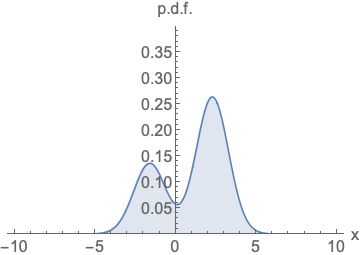
\includegraphics[width=\textwidth]{ProbabilityDensityFunctions.png}
						\caption{\scriptsize Phải chuẩn hoá (diện tích dưới đường cong phải tích phân thành một)}
					\end{figure}
				\end{column}
				\begin{column}{0.5\textwidth}
					\begin{figure}
						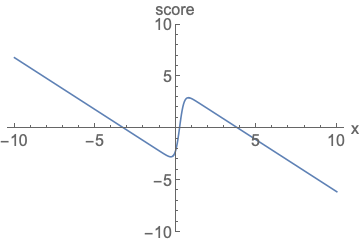
\includegraphics[width=\textwidth]{ScoreFunction.png}
						\caption{\scriptsize Không cần chuẩn hoá.}
					\end{figure}
				\end{column}
			\end{columns}
			
			
			
			\begin{columns}
				\begin{column}{0.5\textwidth}
					\centering
					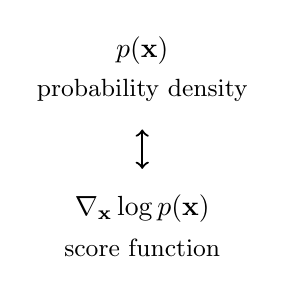
\begin{tikzpicture}
						\node at (0, 1) {$p(\mathbf{x})$};
						
						\node at (0, 0.5) {\small \text{probability density}};
						
						\draw[<->, thick] (0, 0) -- (0, -0.5);
						
						\node at (0, -1) {$\nabla_\mathbf{x} \log p(\mathbf{x})$};
						
						\node at (0, -1.5) {\small \text{score function}};
					\end{tikzpicture}
					
				\end{column}
				\begin{column}{0.5\textwidth}
					\begin{figure}
						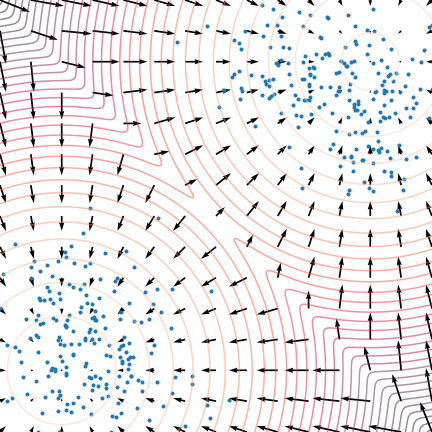
\includegraphics[width=\textwidth]{CompareScoreFunction.png}
						\caption{\scriptsize score function vs probability density}
					\end{figure}
				\end{column}
			\end{columns}
		\end{column}
	\end{columns}	
\end{frame}


\begin{frame}{Diffuse và Denoise thông thường}
%\begin{columns}
%	\begin{column}[T]{0.5\textwidth}
%	
%	\end{column}
%	
%	\hspace*{-1em}
%	
%	\begin{column}[T]{0.5\textwidth}
%		
%	\end{column}
%\end{columns}

\textbf{Diffuse}: Cho $\{\alpha_t \in (0, 1)\}_{t=1}^T$ và $\alpha_1 > \alpha_2 > \dots > \alpha_T$.

Với nhiễu:  $\boldsymbol{\epsilon}_{0}, \boldsymbol{\epsilon}_{1}, \dots \boldsymbol{\epsilon}_{T} \sim \mathcal{N}(\mathbf{0}, \mathbf{I});$
$\boldsymbol{\epsilon}_i \neq \boldsymbol{\epsilon}_j \ (\forall i, j \in T) $, nhiễu $\epsilon_t$ cố định.
\vspace{-25pt}

\begin{equation}
	\mathbf{x}_t=\sqrt{\alpha_t} \cdot \mathbf{x}_{t-1}+\sqrt{1 - \alpha_t} \cdot \epsilon
\end{equation}
\vspace{-15pt}

%	\[
%	q(x_t | x_{t-1}) = \mathcal{N}(x_t; \sqrt{1 - \beta_t} \, x_{t-1}, \beta_t \, I)
%	\]
\begin{figure}
	\centering
	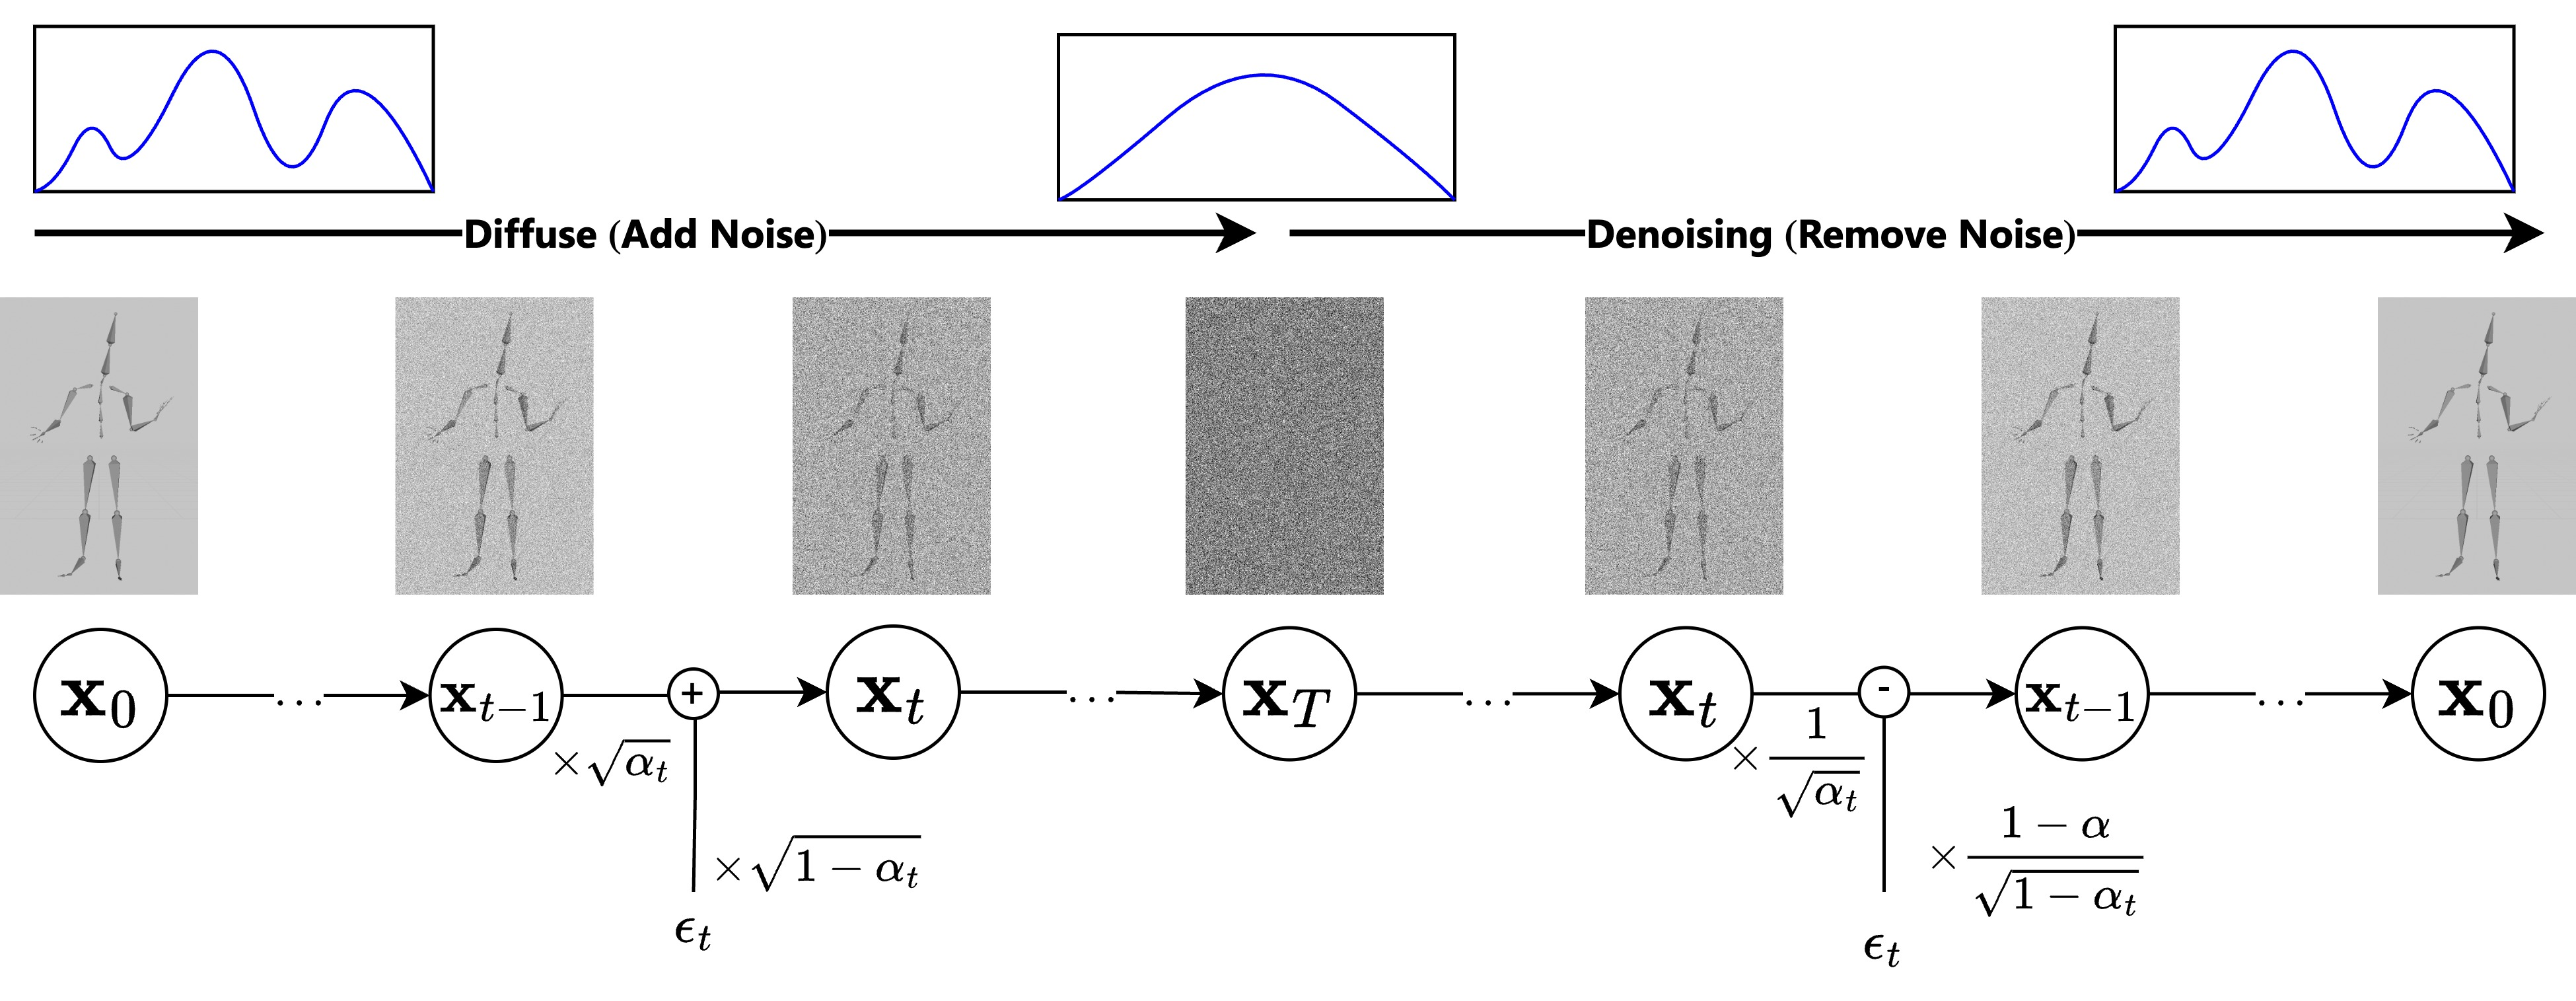
\includegraphics[width=\textwidth]{DiffuseAndDenoise.jpg}
\end{figure}
%\begin{equation}
%	\mathbf{x}_{t-1}=\frac{1}{\sqrt{\alpha_t}}\left(\bx_t-\sqrt{1 - \alpha_t} \cdot \epsilon (\mathbf{x}_t, t )\right)
%\end{equation}

\begin{columns}
	\begin{column}{0.5\textwidth}
		\textbf{Denoise}
		\begin{equation}
			\mathbf{x}_{t-1} = \frac{1}{\sqrt{\alpha_{t}}} (\mathbf{x}_t - \sqrt{1- \alpha_t} \cdot \epsilon)
		\end{equation}
	\end{column}
	\begin{column}{0.5\textwidth}
	\begin{figure}
		\centering
		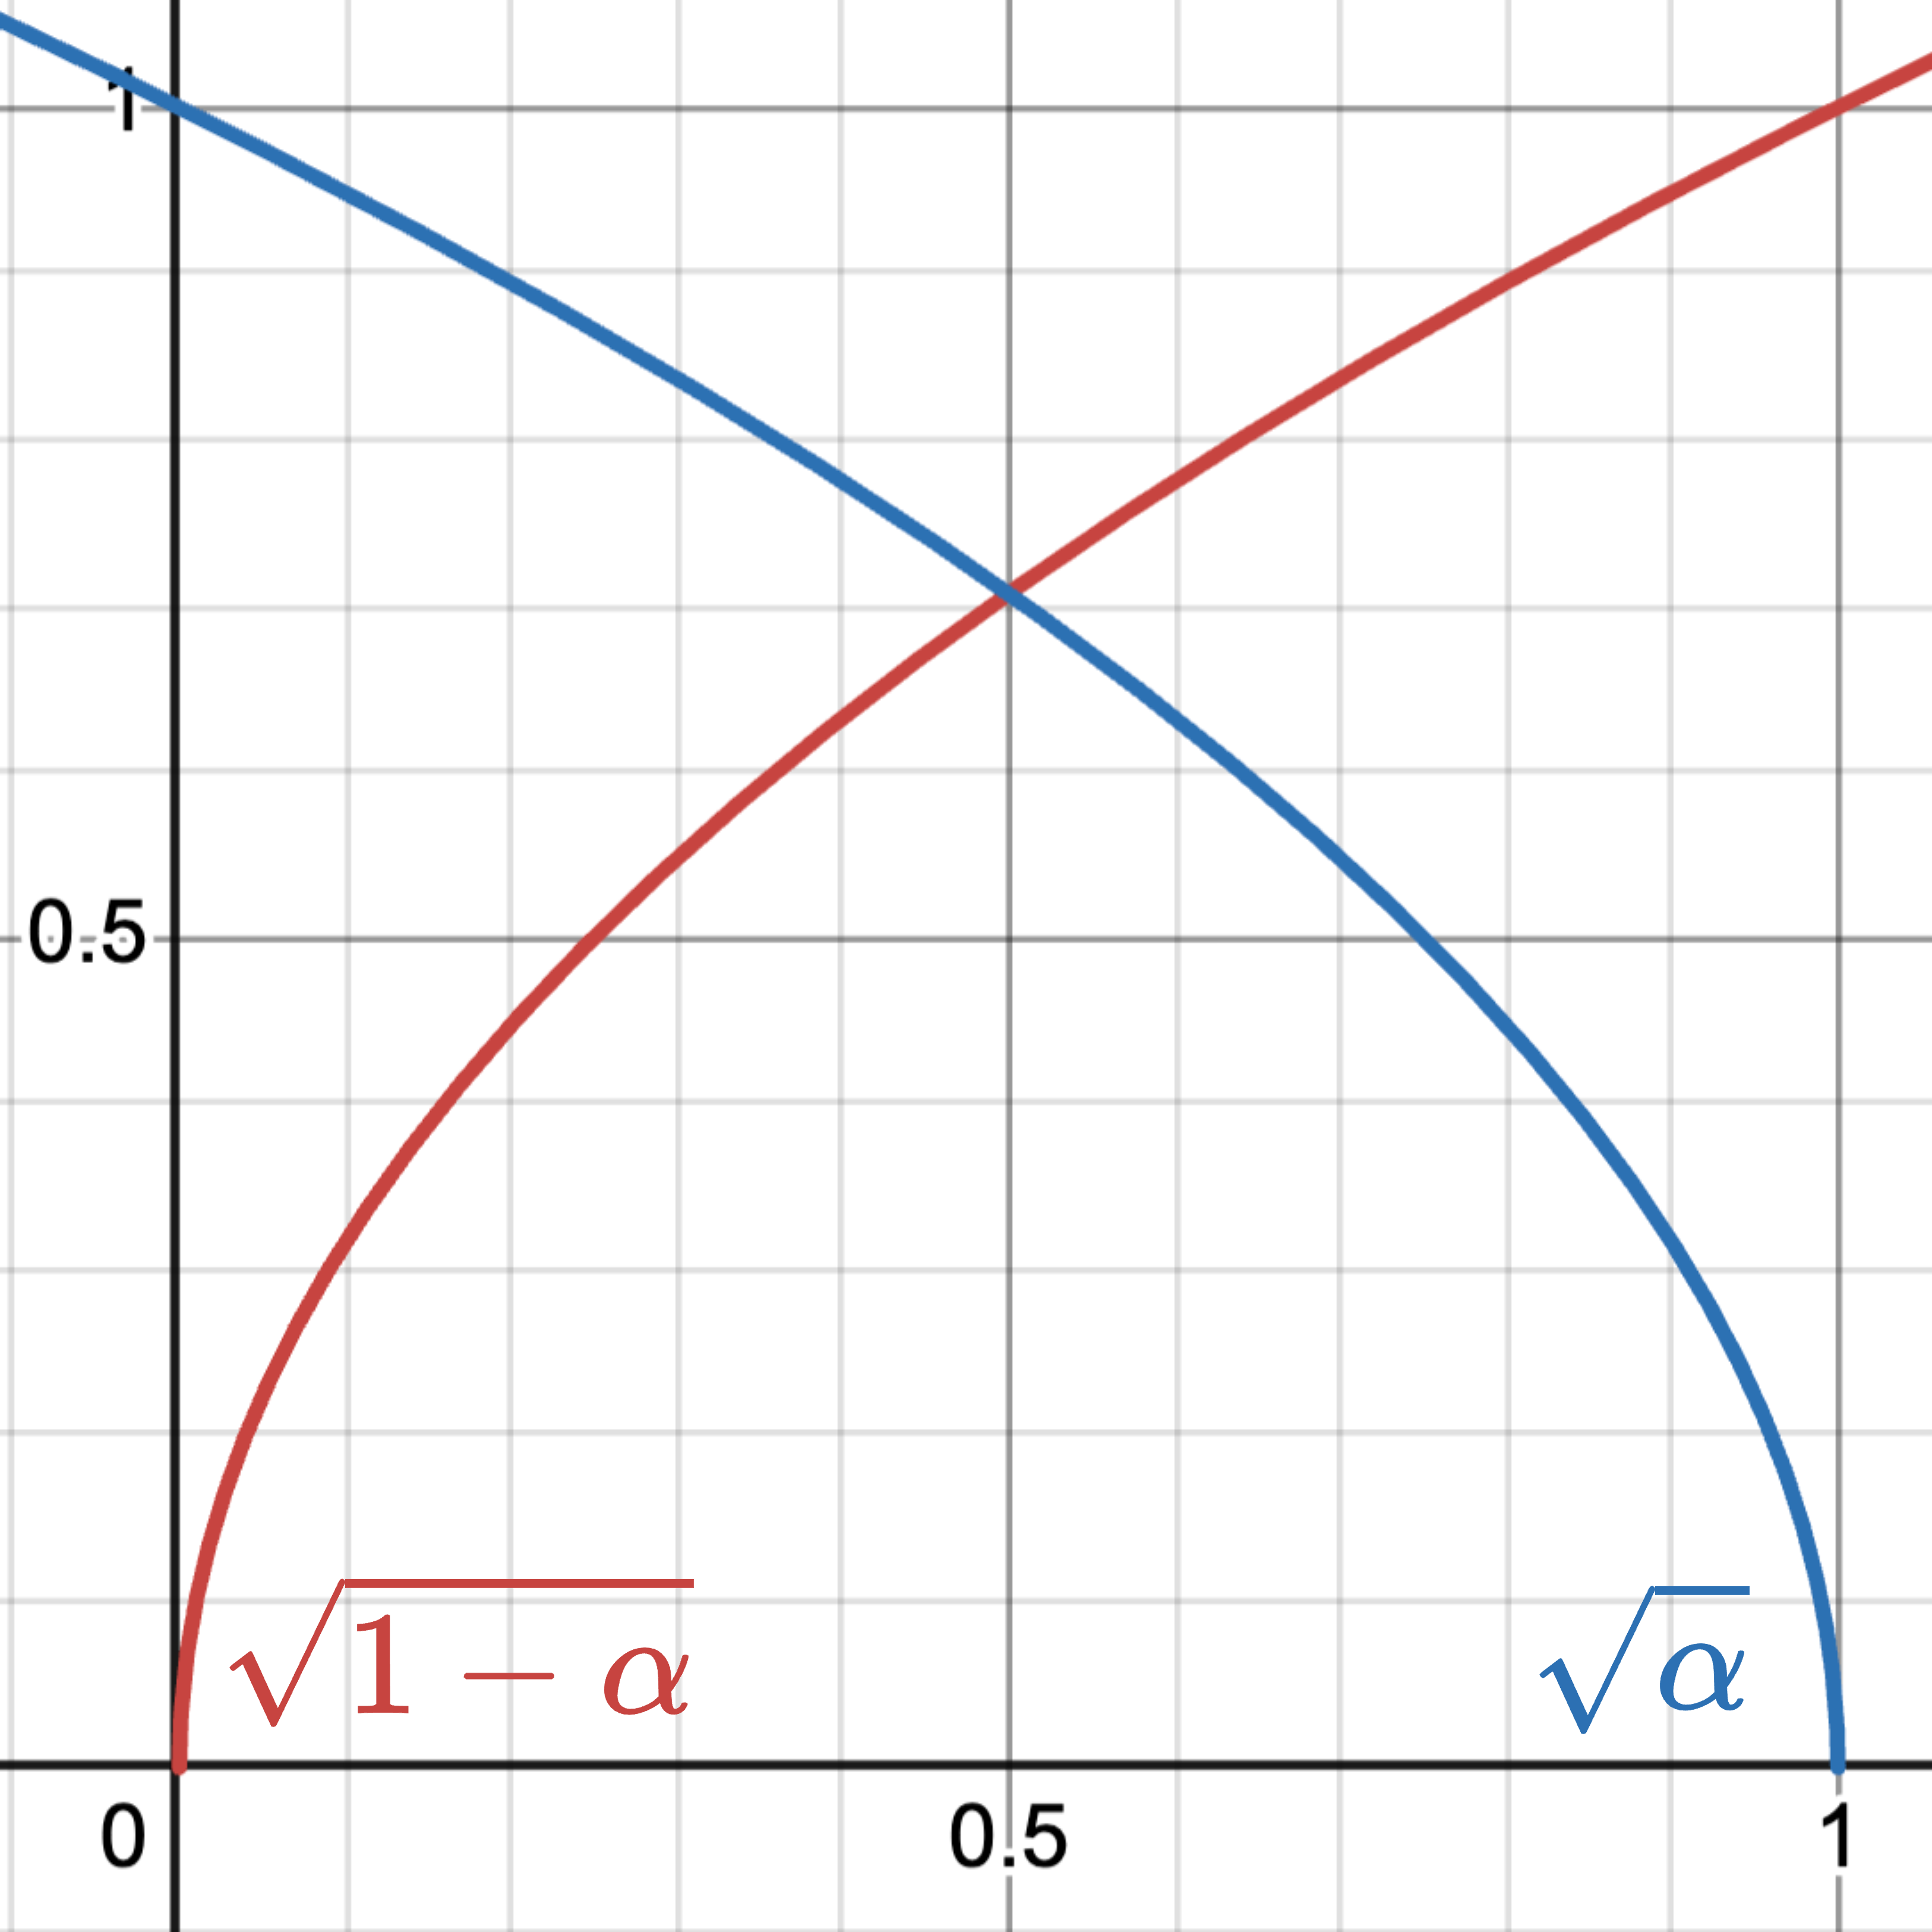
\includegraphics[width=0.4\textwidth]{SquareAlpha.png}
	\end{figure}
	\end{column}
\end{columns}

\end{frame}


\begin{frame}{Quan hệ $\bx_t$ và $\bx_{t - 1}$}
	
	Ta có thể suy ra $\bx_t$ từ $\bx_0$ và ngược lại. Với $ \boldsymbol{\epsilon}_{t-1}, \boldsymbol{\epsilon}_{t-2}, \dots \sim \mathcal{N}(\mathbf{0}, \mathbf{I})$
	%\begin{align*}
	%	\mathbf{x}_t & = \sqrt{\alpha_t}\mathbf{x}_{t-1} + \sqrt{1 - \alpha_t} \boldsymbol{\epsilon}_{t-1} \\
	%	& = \sqrt{\alpha_t \alpha_{t-1}} \mathbf{x}_{t-2} + \sqrt{1 - \alpha_t \alpha_{t-1}} \bar{\boldsymbol{\epsilon}}_{t-2} \\
	%	& = \dots \\
	%	& = \sqrt{\bar{\alpha}_t}\mathbf{x}_0 + \sqrt{1 - \bar{\alpha}_t}\boldsymbol{\epsilon}
	%\end{align*}
	\vspace{-10pt}
	
	\begin{figure}
		\centering
		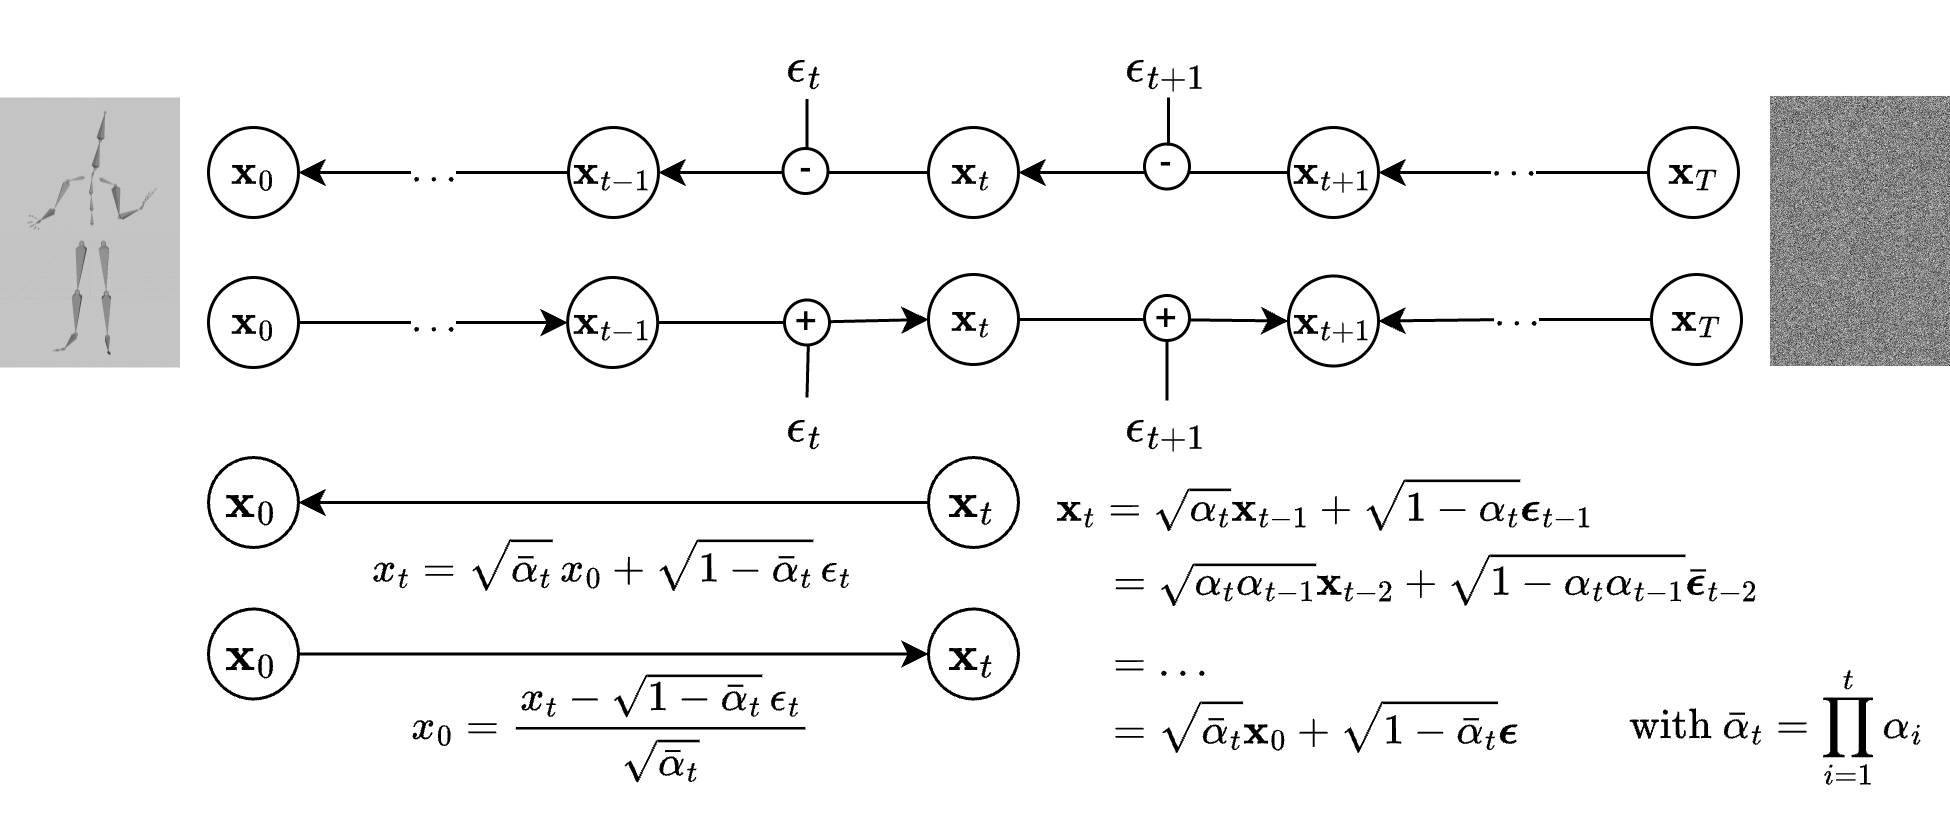
\includegraphics[width=\textwidth]{XRelation.png}
	\end{figure}
	%\vspace{-10pt}
	%	\mathbf{x}_t = \sqrt{\bar{\alpha}_t}\mathbf{x}_0 + \sqrt{1 - \bar{\alpha}_t}\boldsymbol{\epsilon}
	\begin{columns}
		\begin{column}{0.5\textwidth}
			\begin{itemize}
				\item $\bar{\alpha}_1 > \dots > \bar{\alpha}_T$
				\item Tổng hai nhiễu cũng là nhiễu:
				\footnotesize
				$$
				\mathcal{N}(\mathbf{0}, \sigma_1^2\mathbf{I}) + 
				\mathcal{N}(\mathbf{0}, \sigma_2^2\mathbf{I})
				=\mathcal{N}(\mathbf{0}, (\sigma_1^2 + \sigma_2^2)\mathbf{I})
				$$
			\end{itemize}
		\end{column}
		\begin{column}{0.5\textwidth}
			
			\begin{figure}
				\centering
				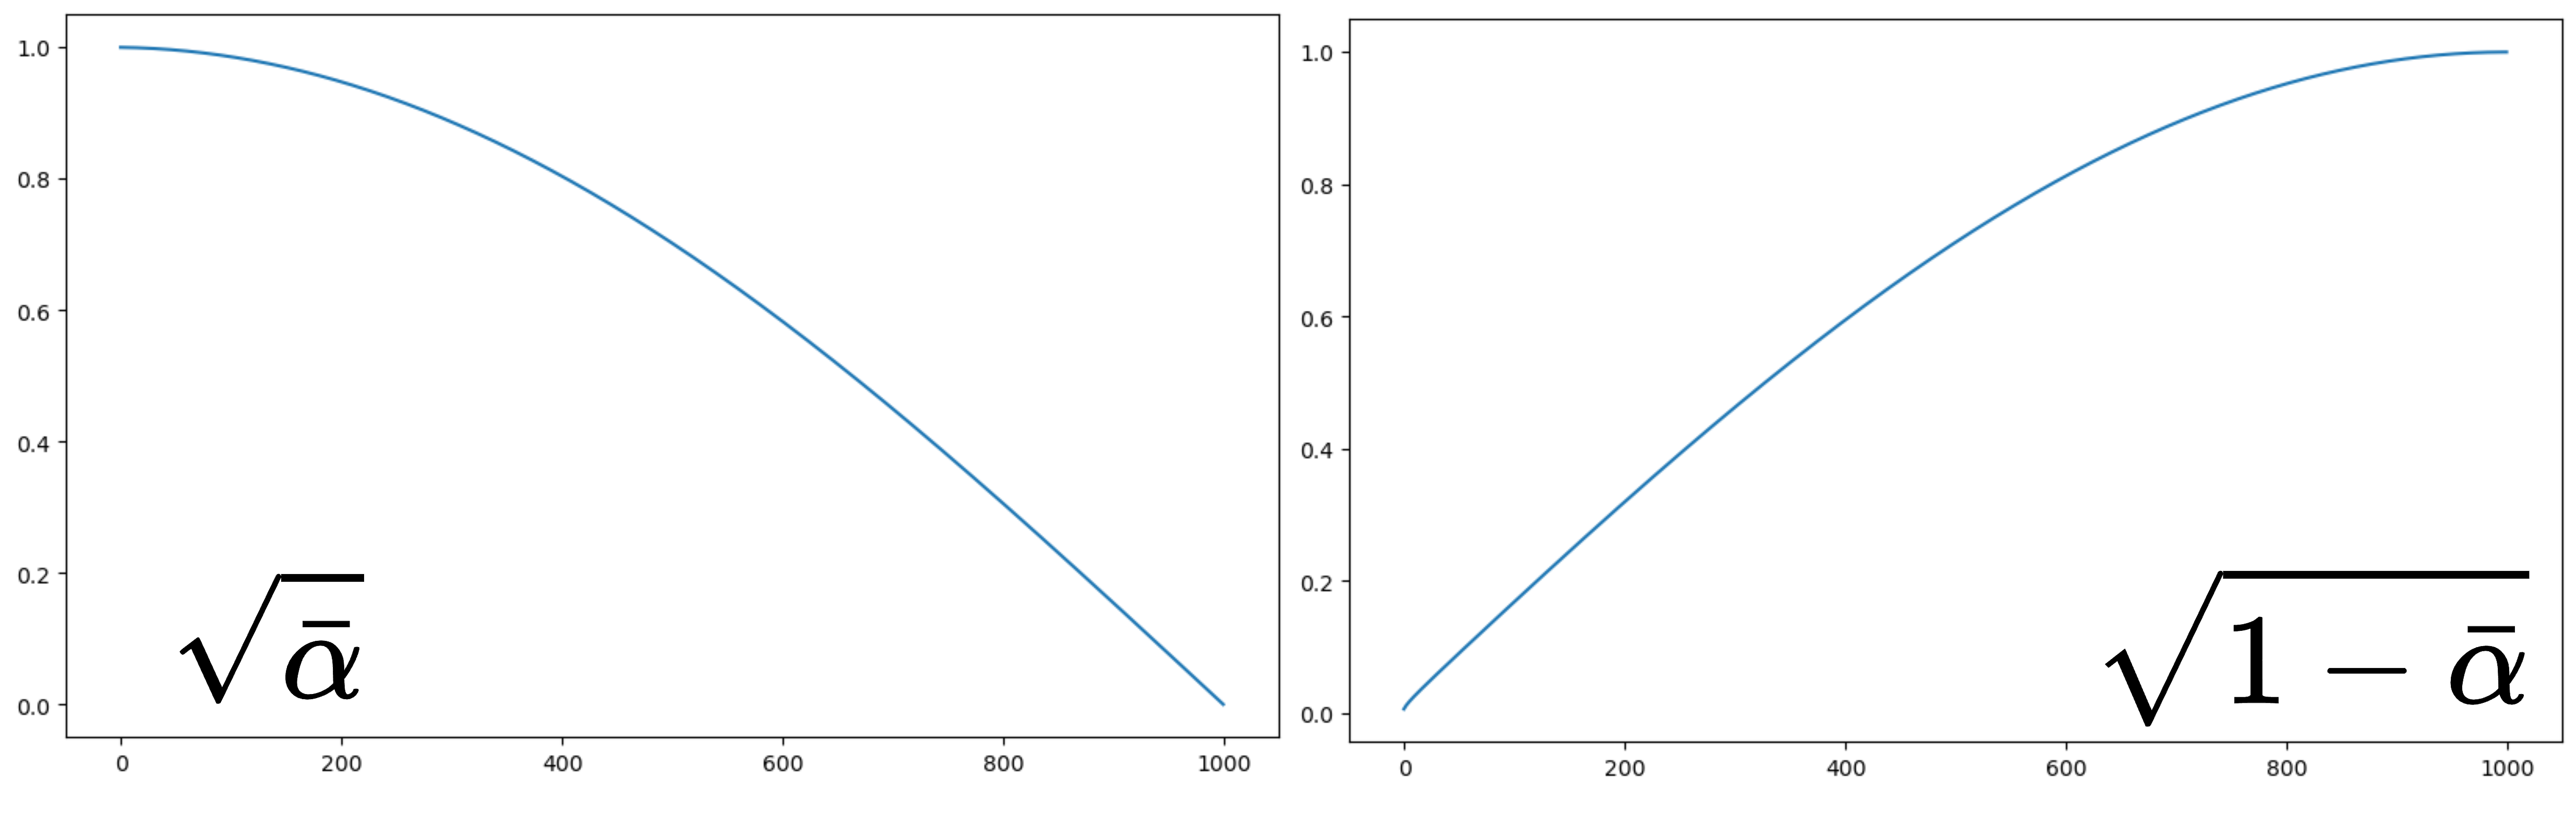
\includegraphics[width=\textwidth]{AlphaCumprod}
			\end{figure}
			
			
		\end{column}
	\end{columns}
	
\end{frame}


\begin{frame}{$q(\bx_t | \bx_{t-1})$ và $p_{\theta}(\bx_{t-1} | \bx_t ) $  trong DDPM }
	\textbf{DDPM} (Denoising Diffusion Probabilistic Model)
\begin{figure}
	\centering
	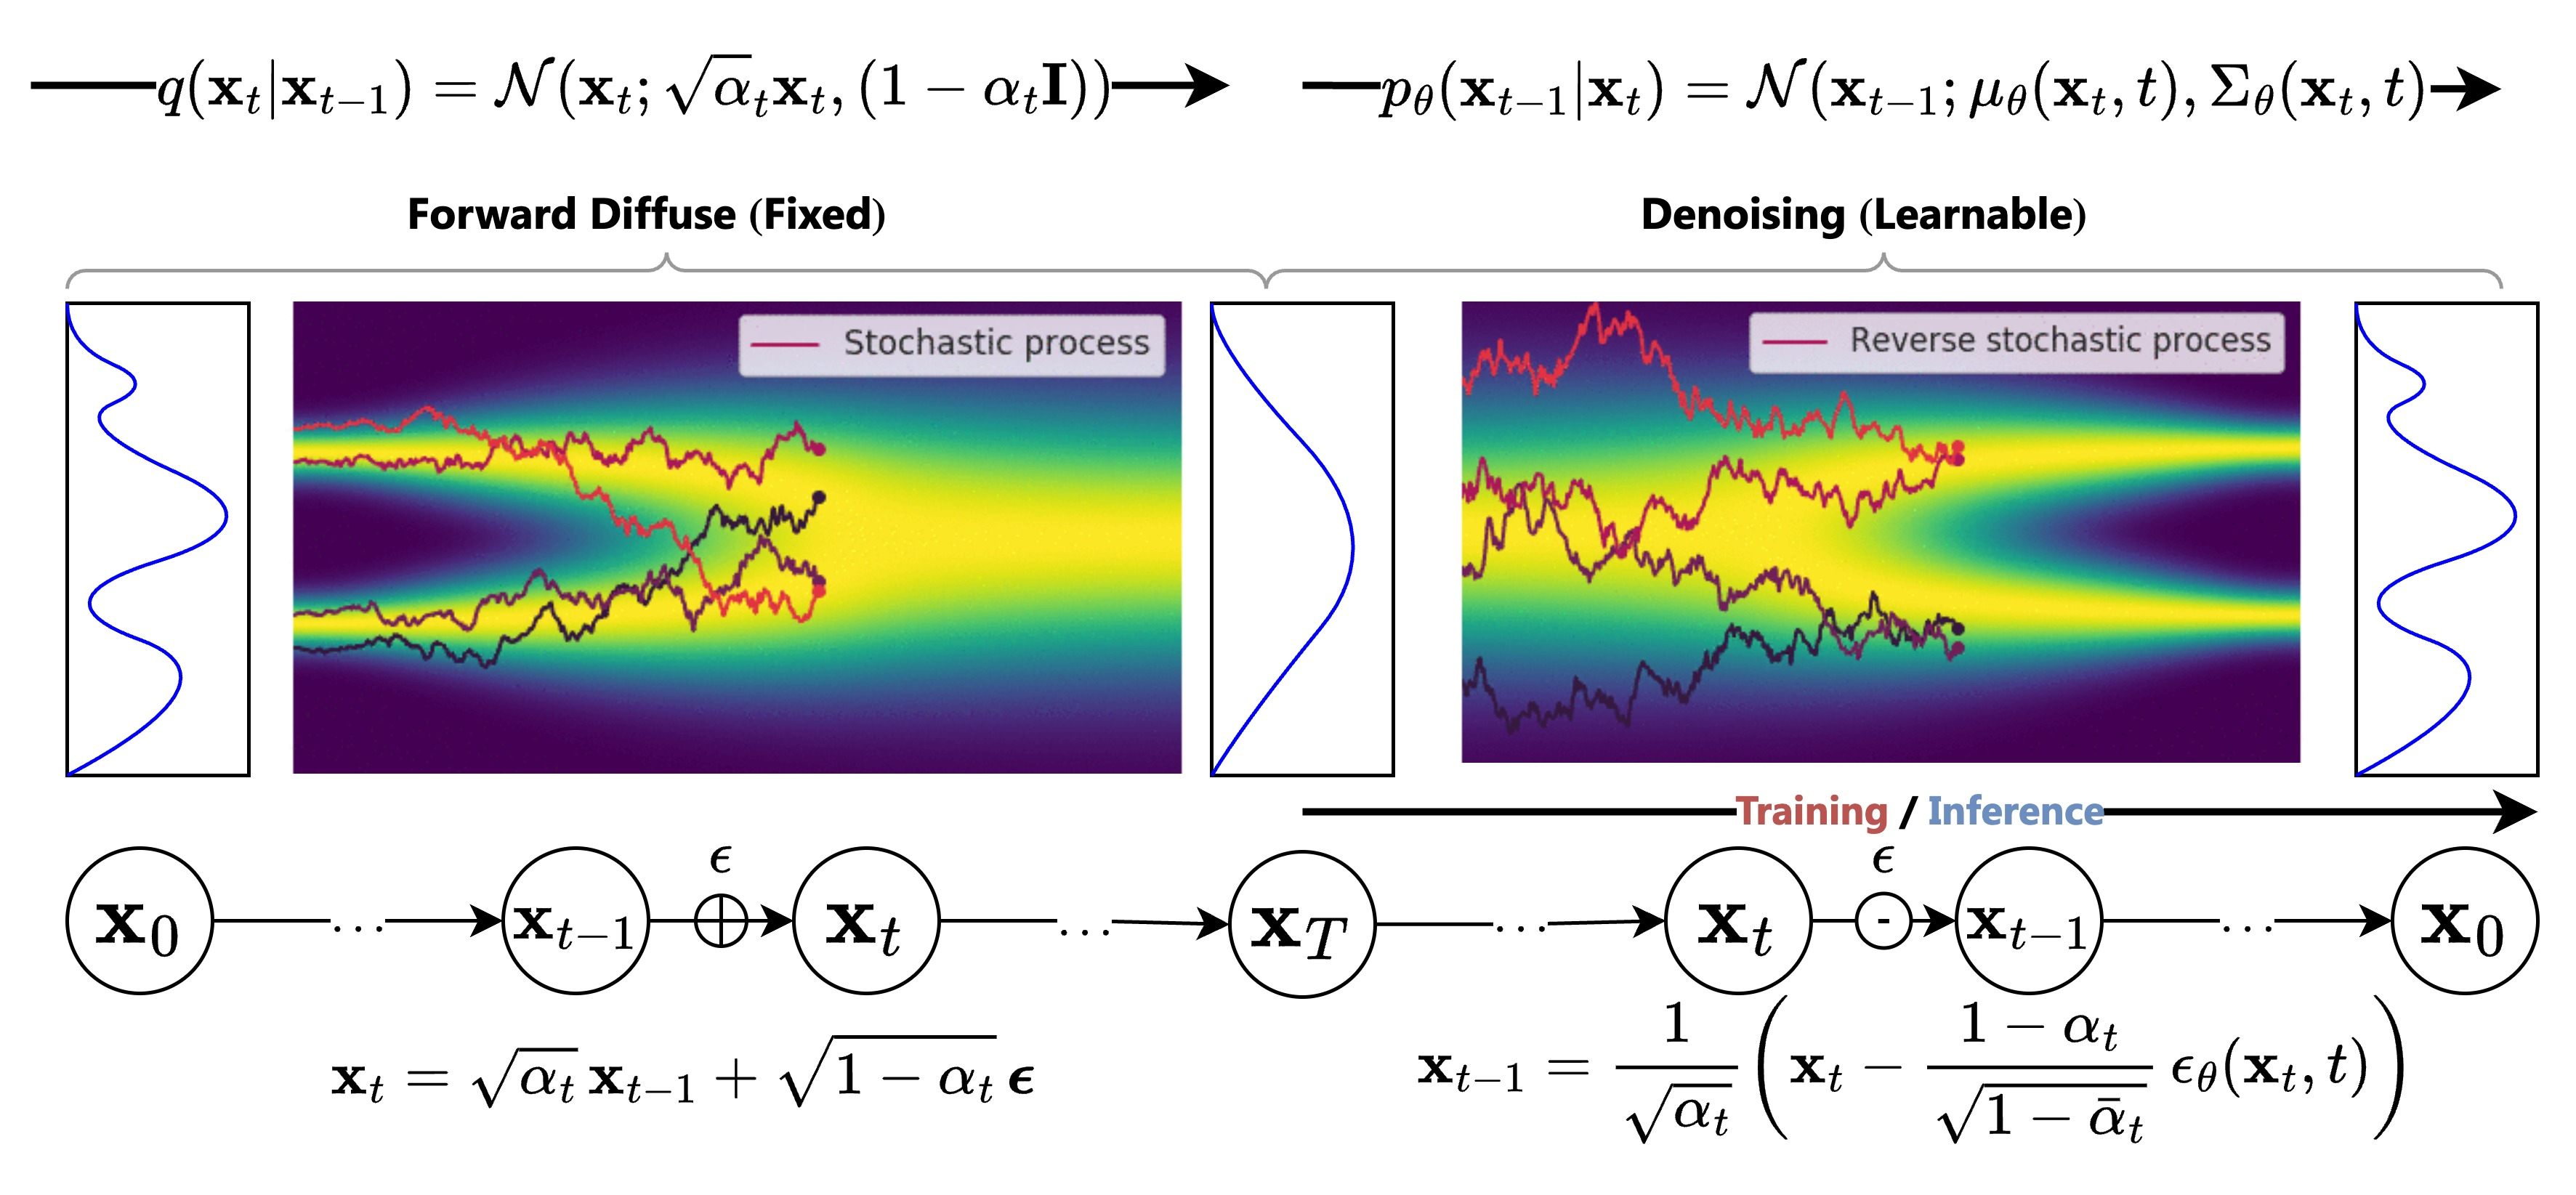
\includegraphics[width=\textwidth]{PQ}
\end{figure}
	
\begin{itemize}
	\item $q (\mathbf{x}_{t} | \mathbf{x}_{t-1}) = \mathcal{N}(\mathbf{x}_t; \sqrt{\alpha}_t \mathbf{x}_t, (1 - \alpha_t \mathbf{I}))$
	\item $p_\theta (\mathbf{x}_{t-1} | \mathbf{x}_{t}) = \mathcal{N}(\mathbf{x}_{t-1}; \mu_\theta{(\mathbf{x}_t, t)}, {\Sigma}_{\theta} {  (\mathbf{x}_t, t ) }$
\end{itemize}
%	$q(\mathbf{x}_t \vert \mathbf{x}_0) = \mathcal{N}(\mathbf{x}_t; \sqrt{\bar{\alpha}_t} \mathbf{x}_0, (1 - \bar{\alpha}_t)\mathbf{I})$
%
%
%
%\begin{equation}
%	\mathbf{x}_{t-1}=\frac{1}{\sqrt{1- \beta_t}}\left(\bx_t-\sqrt{\beta_t} \cdot \epsilon_{\color{red}{\theta}}\left(\mathbf{x}_t, t\right)\right)+\color{red}{\beta_t \cdot \sigma_t \mathbf{z}} \color{black}{}
%\end{equation}

\end{frame}

\begin{frame}{Vanilla Diffusion với $\epsilon$ Objective}
	\begin{figure}
		\centering
		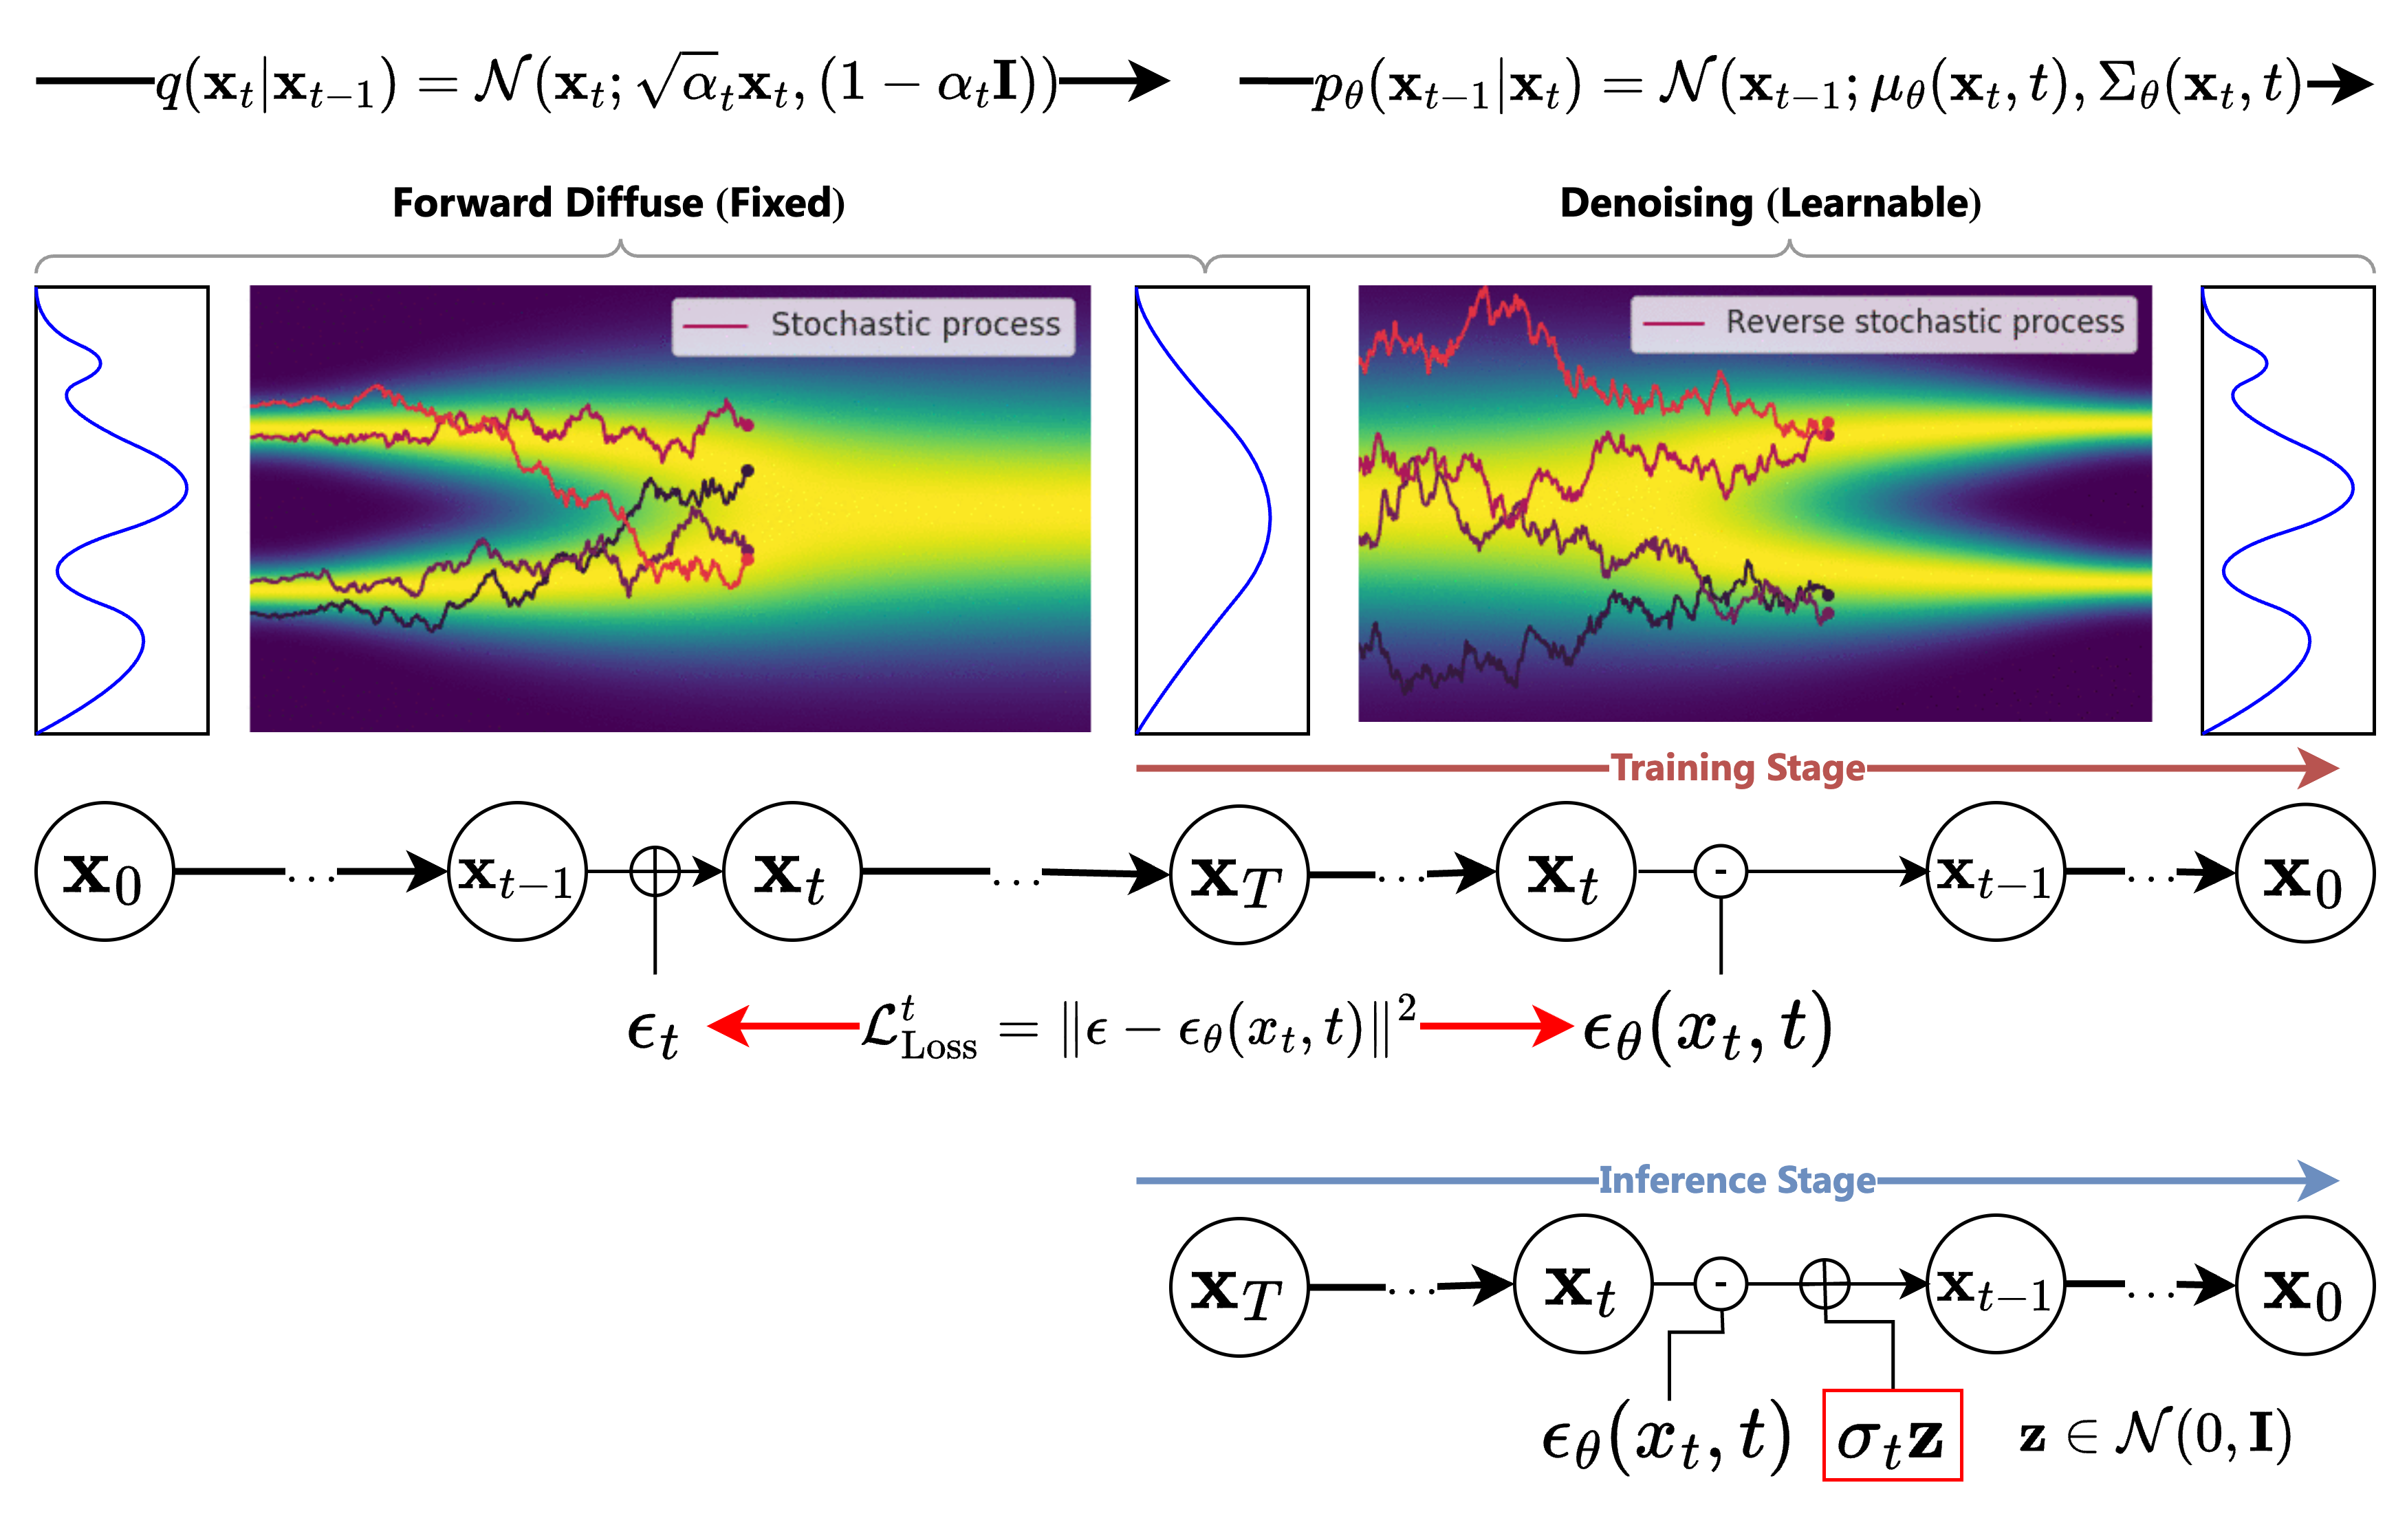
\includegraphics[width=0.95\textwidth]{TrainingAndSamplingStandard.png}
	\end{figure}
\end{frame}

\begin{frame}{Điều khiển $\sigma_t$ bằng với Langevin dynamics}
%	Cho $L$ là biến điều chỉnh độ lệch chuẩn
	%	 $\mathcal{N}(0, \sigma_i^2 I), i=1,2,\cdots,L$. $\mathbf{s}_\theta(\mathbf{x}, i) \approx \nabla_\mathbf{x} \log p_{\sigma_i}(\mathbf{x})$ $i= 1, 2, \cdots, L$.
	
%	Ta dễ dàng sinh mẫu (sampling) từ ${\sigma_i}(\mathbf{x})$ bằng cách lấy mẫu $\mathbf{x} \sim p(\mathbf{x})$  và tính $\mathbf{x} + \sigma_i \mathbf{z}$ với $\mathbf{z} \sim \mathcal{N}(0, I)$
Trong quá trình Denoise ($T \rightarrow 0$)  $\sigma_T > \cdots  >  \sigma_2 > \sigma_1$, ta sẽ giảm $\sigma_t$ để giảm dần nhiễu, để mô hình có thể hội tụ ở những vùng có mật độ xác xuất cao.
	\begin{figure}
		\centering
		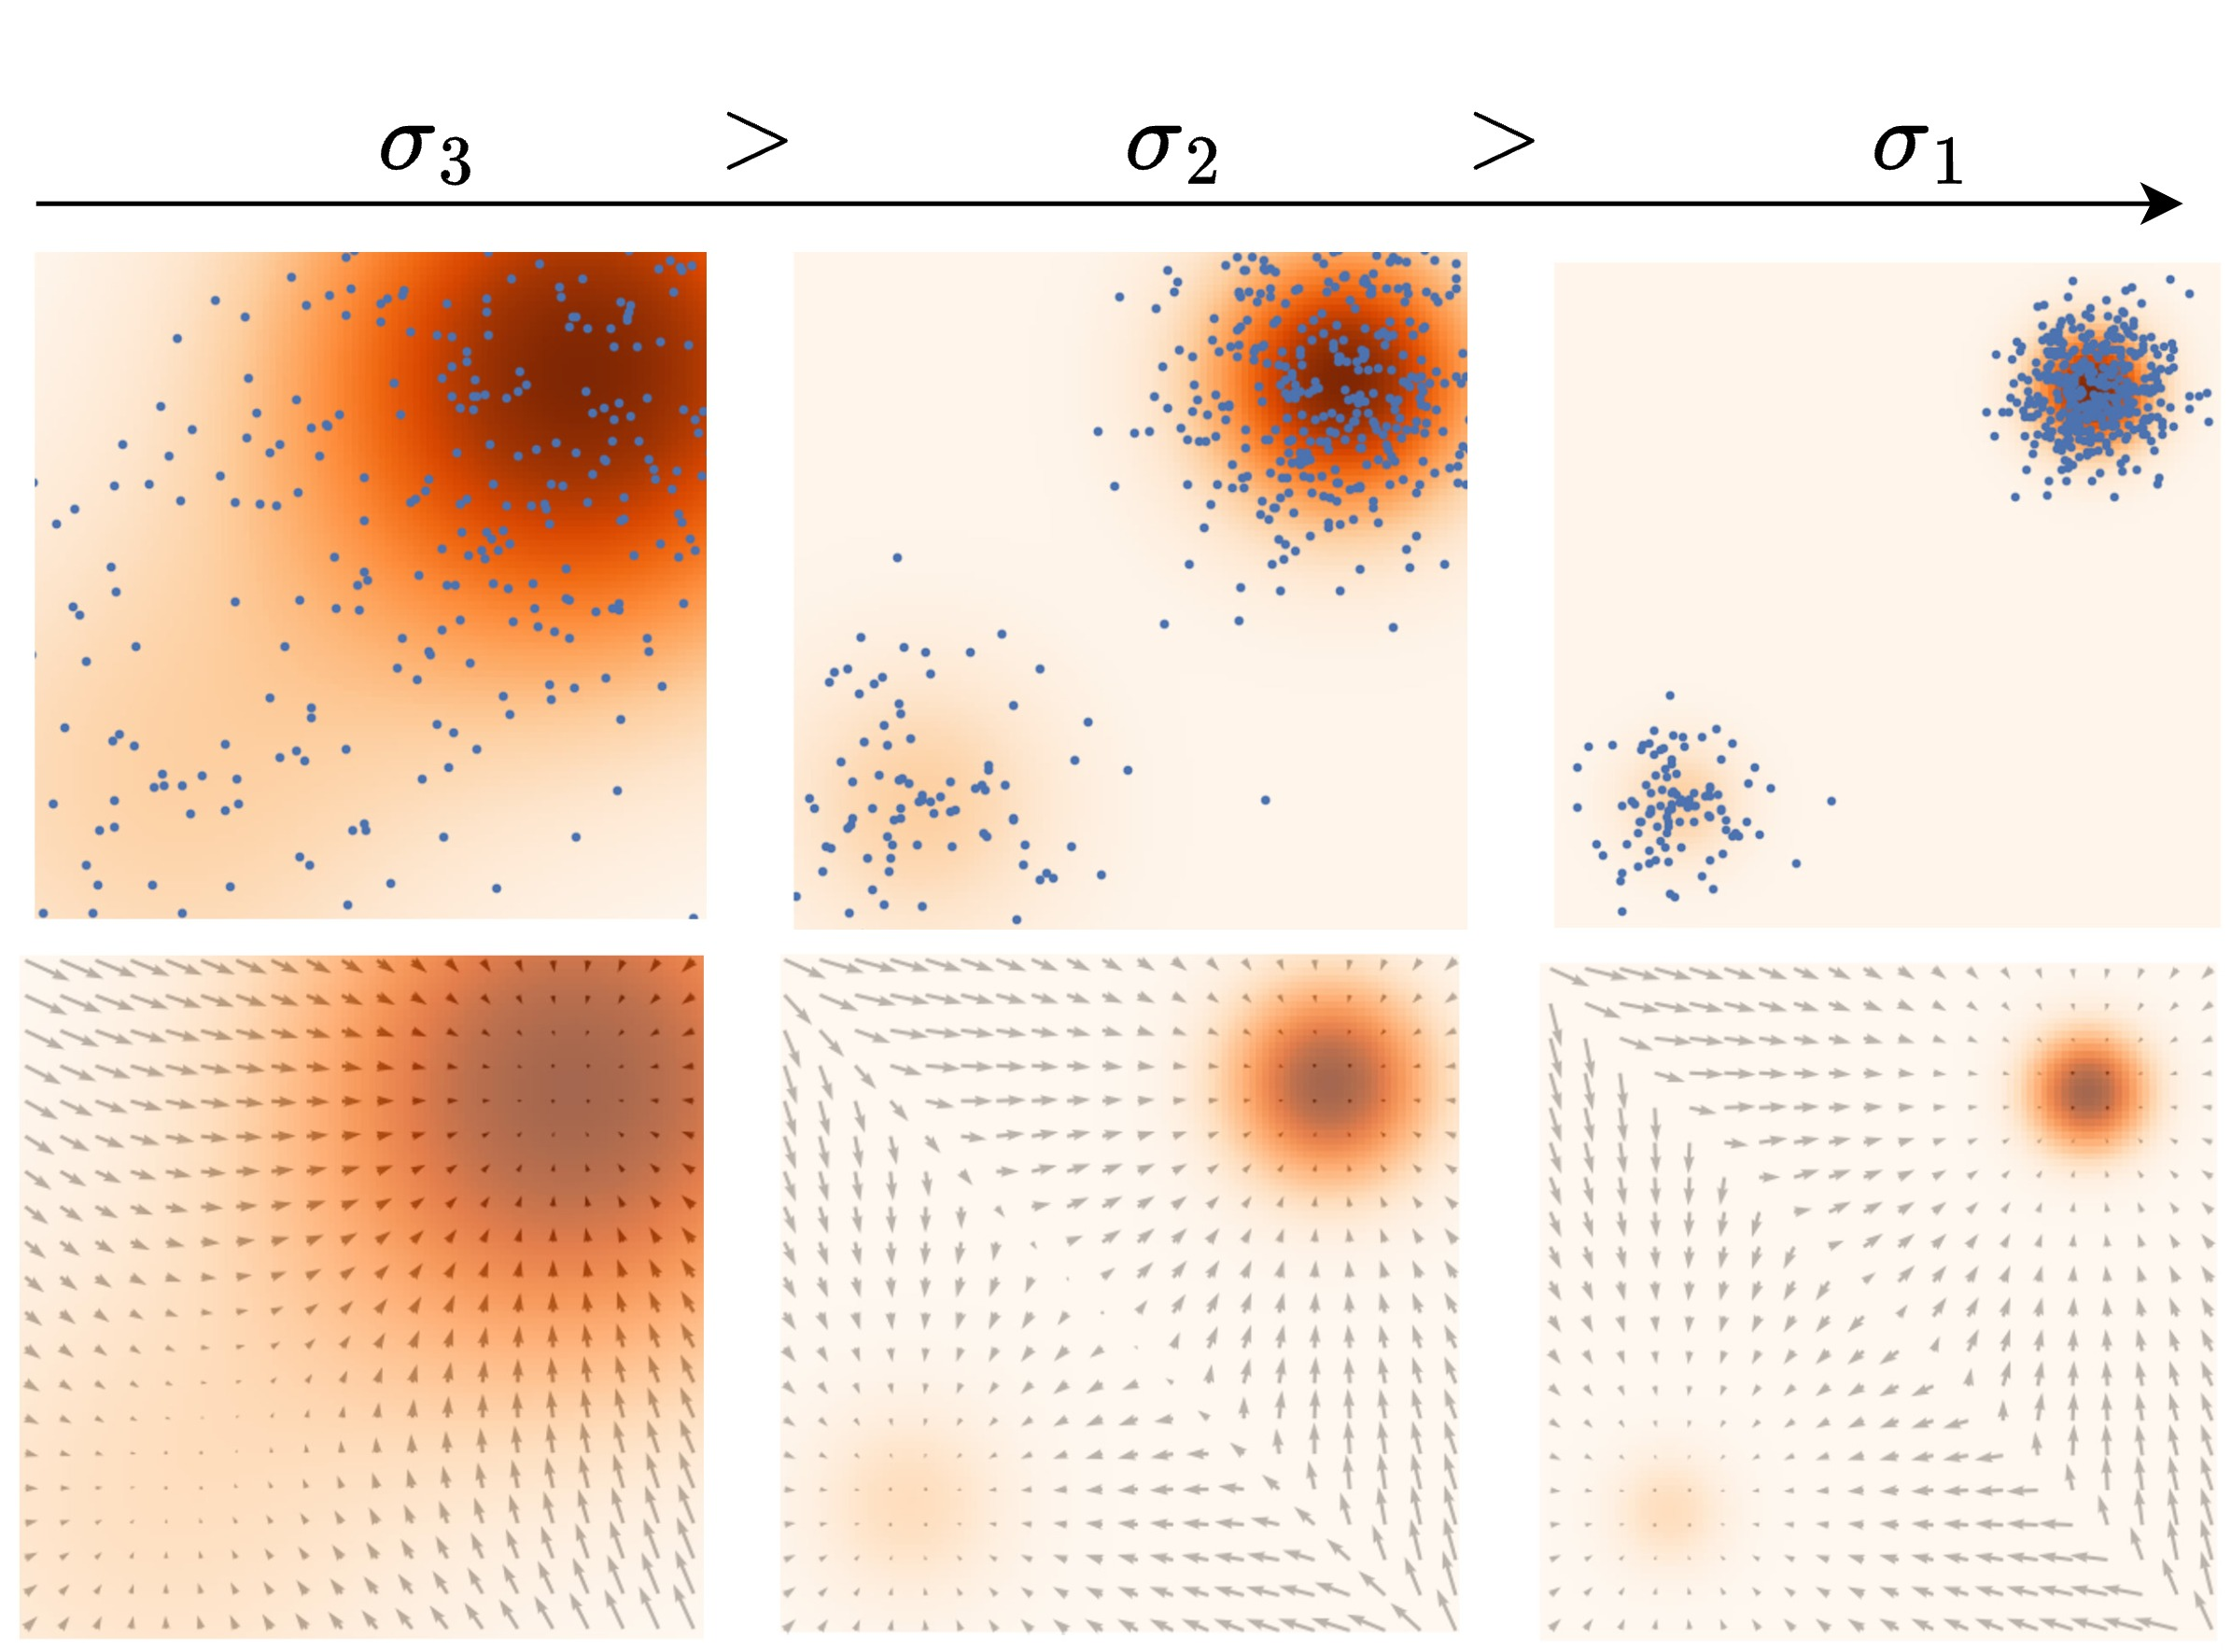
\includegraphics[width=0.8\linewidth]{NoiseScale.jpg}
	\end{figure}
\end{frame}

\begin{frame}{Training DDPM}
	\textbf{Hàm loss}: $\mathcal{L} = \sum_{t=1}^{T} \mathcal{L}_t$. $\mathcal{L}_{t}= \mathbb{E}_{\mathbf{x}_{0}, \epsilon_t \sim \mathcal{N}(0, I), t} \left[ \| \epsilon_t - \epsilon_\theta(\mathbf{x}_t, t) \|^2 \right]$
	
	\begin{figure}
		\centering
		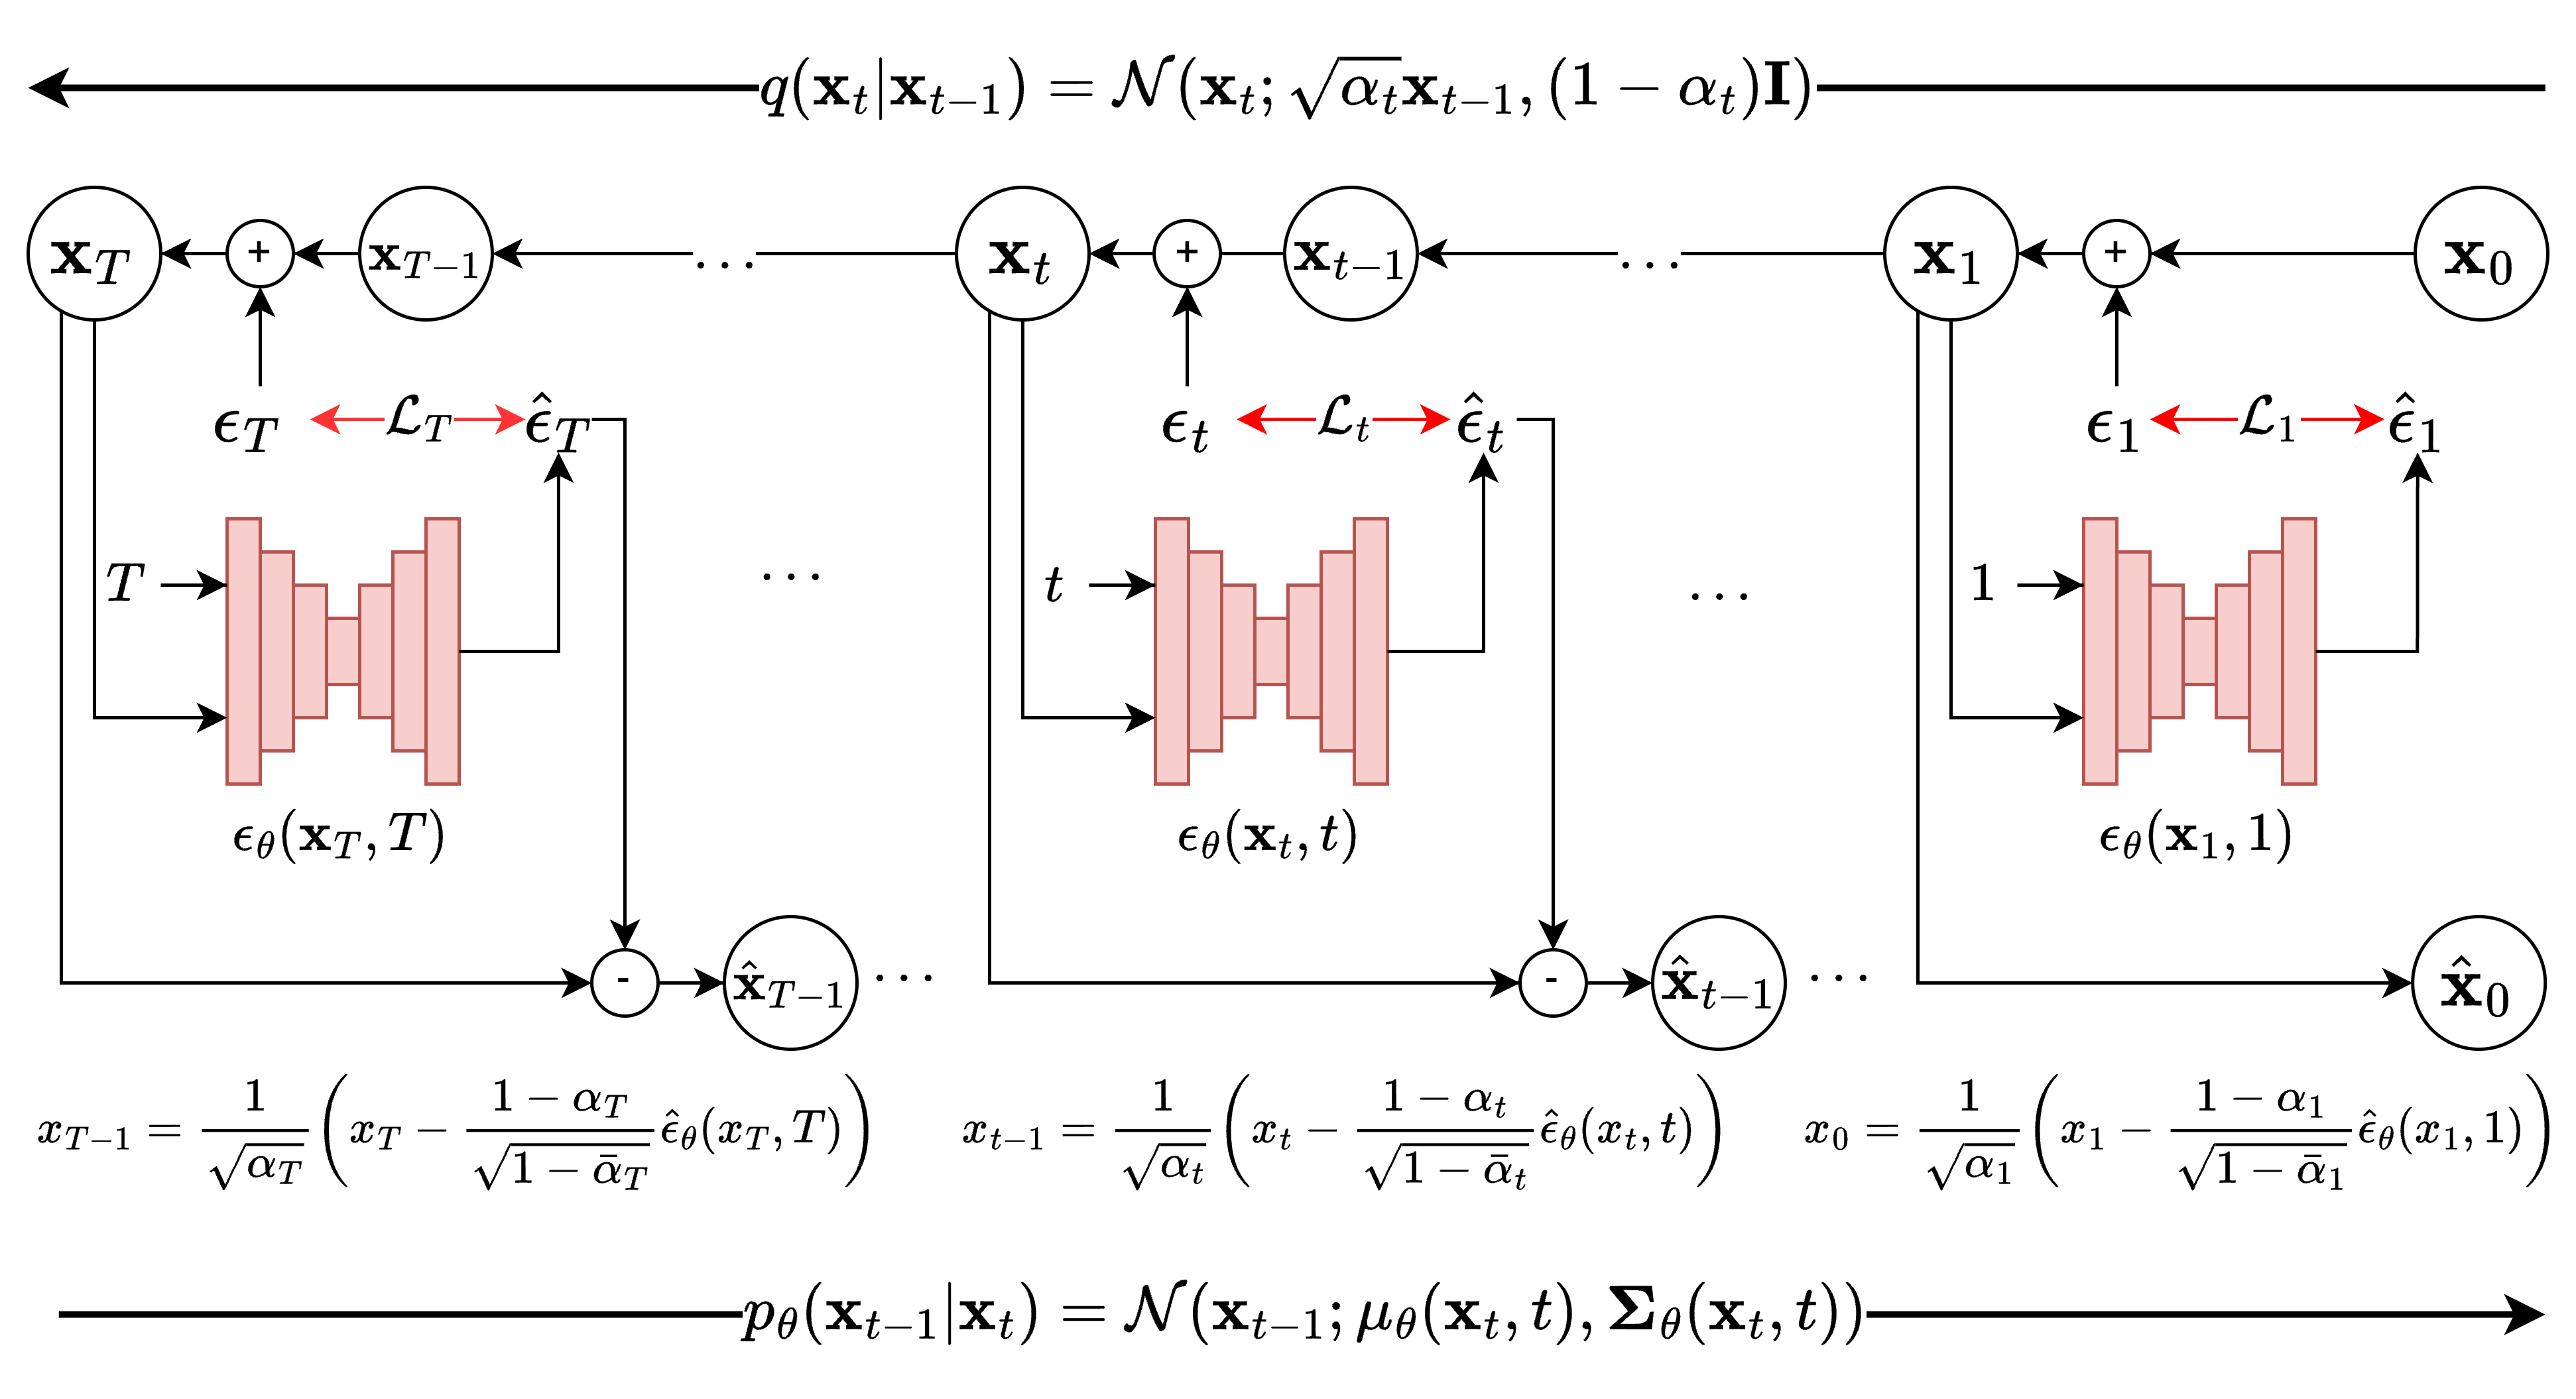
\includegraphics[width=\linewidth]{DDPMTraining}
	\end{figure}
\end{frame}

\begin{frame}{Các bước huấn luyện với DDPM}
	
	\begin{enumerate}
		\item Tính sẵn các giá trị $\sqrt{\alpha_t}$ $\sqrt{1 - \alpha_t}$ và $\sqrt{\bar{\alpha}_t}$ ở mọi bước $t: 1 \rightarrow T$.
		$\{\alpha_t \in (0, 1)\}_{t=1}^T$, $\alpha_1 < \alpha_2 < \dots < \alpha_T$
		\item Lấy nhãn $\bx_0$ từ phân bố của dữ liệu đã chuẩn hoá
		\item Random nhiễu $\bepsilon_t$ ở mọi bước $t: 1 \rightarrow T$, với  $\forall t:  \bepsilon_t \sim\mathcal{N}(\bzero,\bI)$
		\item Gây nhiễu (forward) $\bx_0$ để thu được $\bx_t$ ở mọi bước $t: 1 \rightarrow T$
		$$
		\mathbf{x}_t = \sqrt{\bar{\alpha}_t}\mathbf{x}_0 + \sqrt{1 - \bar{\alpha}_t}\boldsymbol{\epsilon}_t
		$$
		\item $\text{for all}$ $t$, lẫy $t$ \textbf{ngẫu nhiên} $t \sim [1, T]$
		\item Cho $\bx_t$ và $t$ vào mô hình để dự đoán nhiễu $\hat{\bepsilon} = \bepsilon_\theta(\mathbf{x}_t, t)$
		\item Đạo hàm để cập nhật trọng số $\qquad \grad_{\theta_t} \left\| \bepsilon_t - \bepsilon_\theta(\mathbf{x}_t, t) \right\|^2$
		$$
			\mathcal{L}_t = \mathbb{E}_{t \sim [1, T], \mathbf{x}_0, \boldsymbol{\epsilon}_t} \Big[\|\boldsymbol{\epsilon}_t - \boldsymbol{\epsilon}_\theta(\sqrt{\bar{\alpha}_t}\mathbf{x}_0 + \sqrt{1 - \bar{\alpha}_t}\boldsymbol{\epsilon}_t, t)\|^2 \Big]
		$$
		\item Quay lại bước 6 cho đến khi hội tụ để thu được $\theta'$
	\end{enumerate}
\end{frame}

\begin{frame}{Sampling DDPM}
	\textbf{Hàm sampling}:
	\begin{itemize}
		\item $\bx_T \in \mathcal{N}(0, \mathbf{I})$
	\end{itemize}
	
	\begin{equation*}
		x_{t-1} = \frac{1}{\sqrt{\alpha_t}} \left( x_t - \frac{1 - \alpha_t}{\sqrt{1 - \bar{\alpha}_t}} \hat{\epsilon}_{\theta'}(x_t, t) \right) + \sigma_t \mathbf{z}
	\end{equation*}
	
	\begin{itemize}
		\item Diffusion: $\mathcal{L}_{\text{loss}}= \mathbb{E}_{\mathbf{x}_{0}, \epsilon_t \sim \mathcal{N}(0, I), t} \left[ \| \epsilon_t - \epsilon_\theta(\mathbf{x}_t, t) \|^2 \right]$
	\end{itemize}
	\begin{figure}
		\centering
		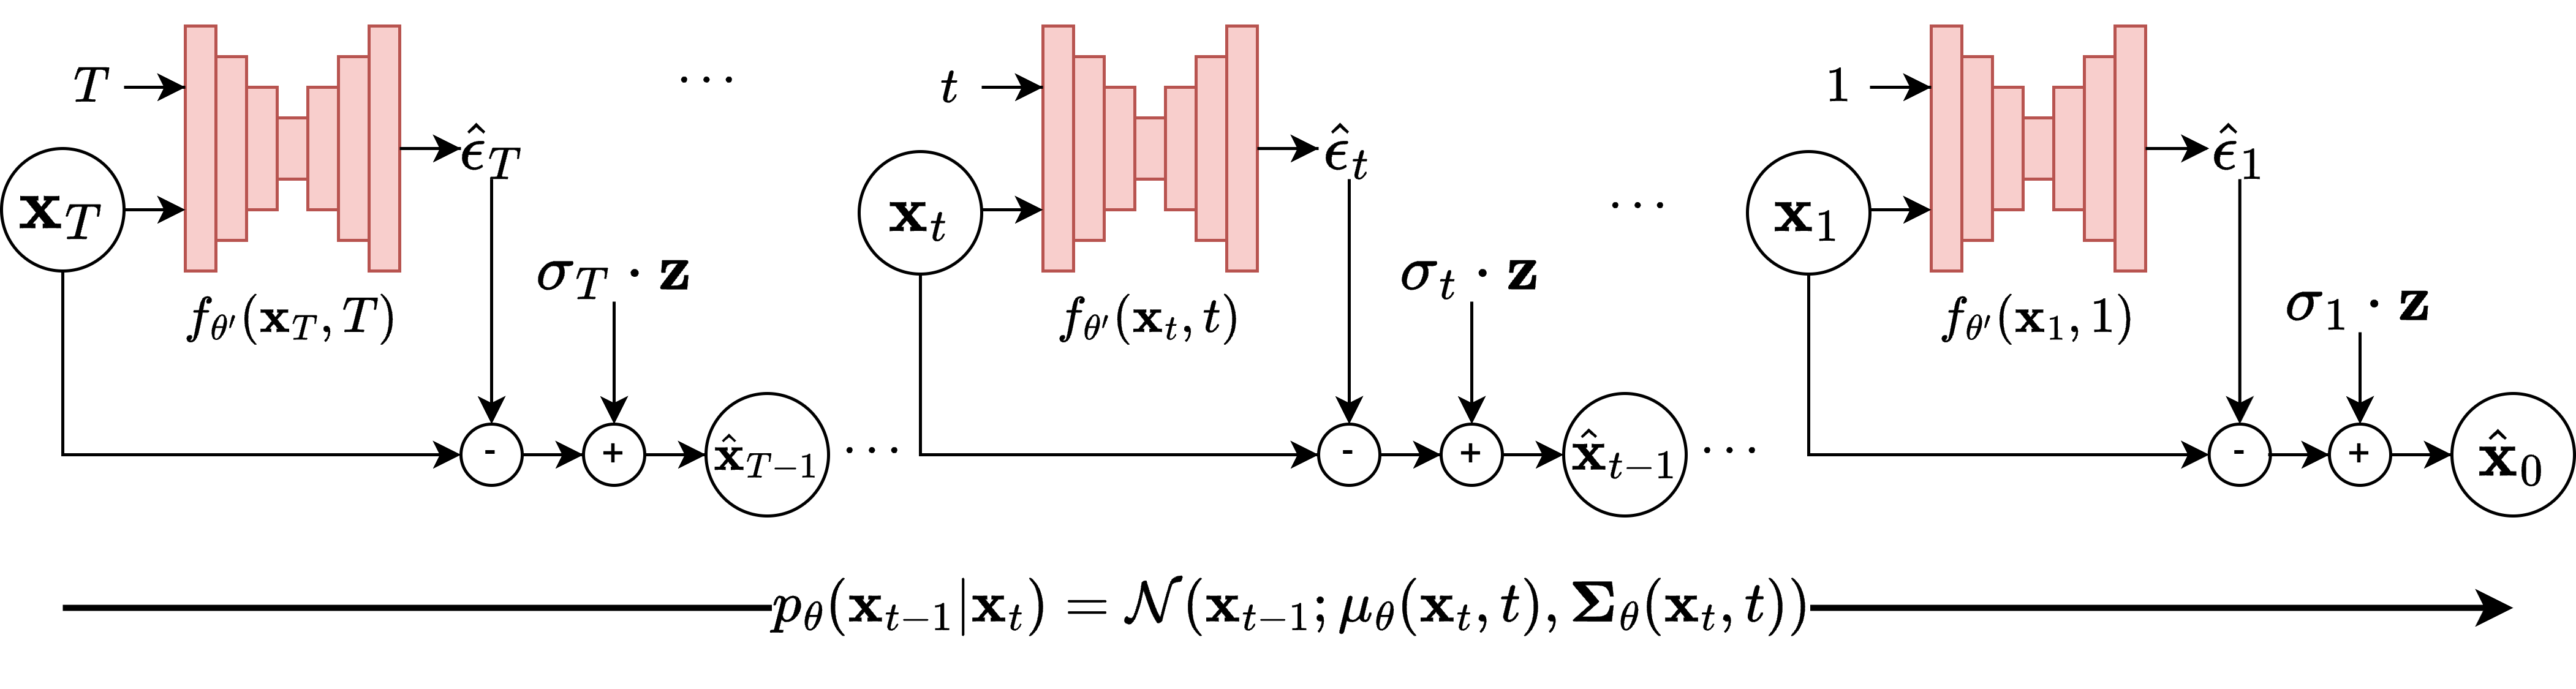
\includegraphics[width=\linewidth]{DDPMSampling}
	\end{figure}
\end{frame}

\begin{frame}{Các bước lấy mẫu với DDPM}
	
	\begin{enumerate}
		\item Bắt đầu với nhiễu: $\bx_T \sim \mathcal{N}(0, \mathbf{I})$
		\item Các giá trị $\sqrt{\alpha_t}$ $\sqrt{1 - \alpha_t}$ và $\sqrt{\bar{\alpha}_t}$ có được từ bước huấn luyện
		\item Tính hệ số điều chỉnh nhiễu $\sigma_t$ từ $\alpha_t$ ở mọi bước $t: 1 \rightarrow T$
		$\sigma_t = \sqrt{\frac{1 - \bar{\alpha}_{t-1}}{1 - \bar{\alpha}_t} (1 - \alpha_t)}$
		
		\item $\text{for all}$ $t$, lấy $t$ \textbf{tuần tự} $t \sim [T, \dots 1]$
		\item Random nhiễu $\bz \sim \mathcal{N}(0, \mathbf{I})$
		\item Đưa $\bx_t$ vào để suy luận nhiễu $\bepsilon_{\theta'} = \bepsilon_{\theta'}(\bx_t, t)$
		\item Dùng nhiễu dự đoán để trừ đi $\bx_t$ ở bước $t$
			$$\mu =  \frac{1}{\sqrt{\alpha_t}}\left( \bx_t - \frac{1-\alpha_t}{\sqrt{1-\bar\alpha_t}} \bepsilon_{\theta'}(\bx_t, t) \right)$$
%			\hat{\bx}_{t-1} =
		\item Cộng thêm một lượng nhiễu $\hat{\bx}_{t-1} = \mu + \sigma_t \bz$
		\item Khi $t=1$ ta thu được $\hat{\bx}_0$ từ quá trình khử nhiễu
	\end{enumerate}
\end{frame}

%	Ta gọi $\epsilon = \mathcal{N}(0, I)$
%\begin{columns}
%\begin{column}{0.8\textwidth}
%\begin{figure}
%	\centering
%	\includegraphics[width=\textwidth]{OverviewDiffusion}
%\end{figure}
%\end{column}
%
%\begin{column}{0.2\textwidth}
%
%\end{column}
%\end{columns}
%\\
%q(\mathbf{x}_t \vert \mathbf{x}_{t-1}) &= \mathcal{N}(\mathbf{x}_t; \sqrt{\alpha_t} \mathbf{x}_{t-1}, (1 - \alpha_t)\mathbf{I}) \\ 
%\rightarrow q(\mathbf{x}_t \vert \mathbf{x}_0) &= \mathcal{N}(\mathbf{x}_t; \sqrt{\bar{\alpha}_t} \mathbf{x}_0, (1 - \bar{\alpha}_t)\mathbf{I})

\begin{frame}{Cải tiến của  với $\mathbf{x}_0$ Objective (DALLE-2)}
	Những điểm cải tiến của $\mathbf{x}_0$ so với $\epsilon$ objective
	\begin{itemize}
		\item Thay vì hàm $f_{\theta}(\bx_t, t)$ dự đoán nhiễu $\epsilon_t$ thì  $f_{\theta}(\bx_t, t)$ dự đoán $\bx_0$.
		\item Sau khi có $\bx_0$ thì ta thêm nhiễu đã có từ trước (từ forward process) để được $\bx_{t-1}$
		\item Tiếp tục cho đến khi được $\hat{\bx}_0$
		
%		$$\tilde{\epsilon}\theta(x_t,t,c) = \epsilon\theta(x_t,t,\emptyset) + w[\epsilon_\theta(x_t,t,c) - \epsilon_\theta(x_t,t,\emptyset)]$$
	\end{itemize} 
	
	\begin{figure}
		\centering
		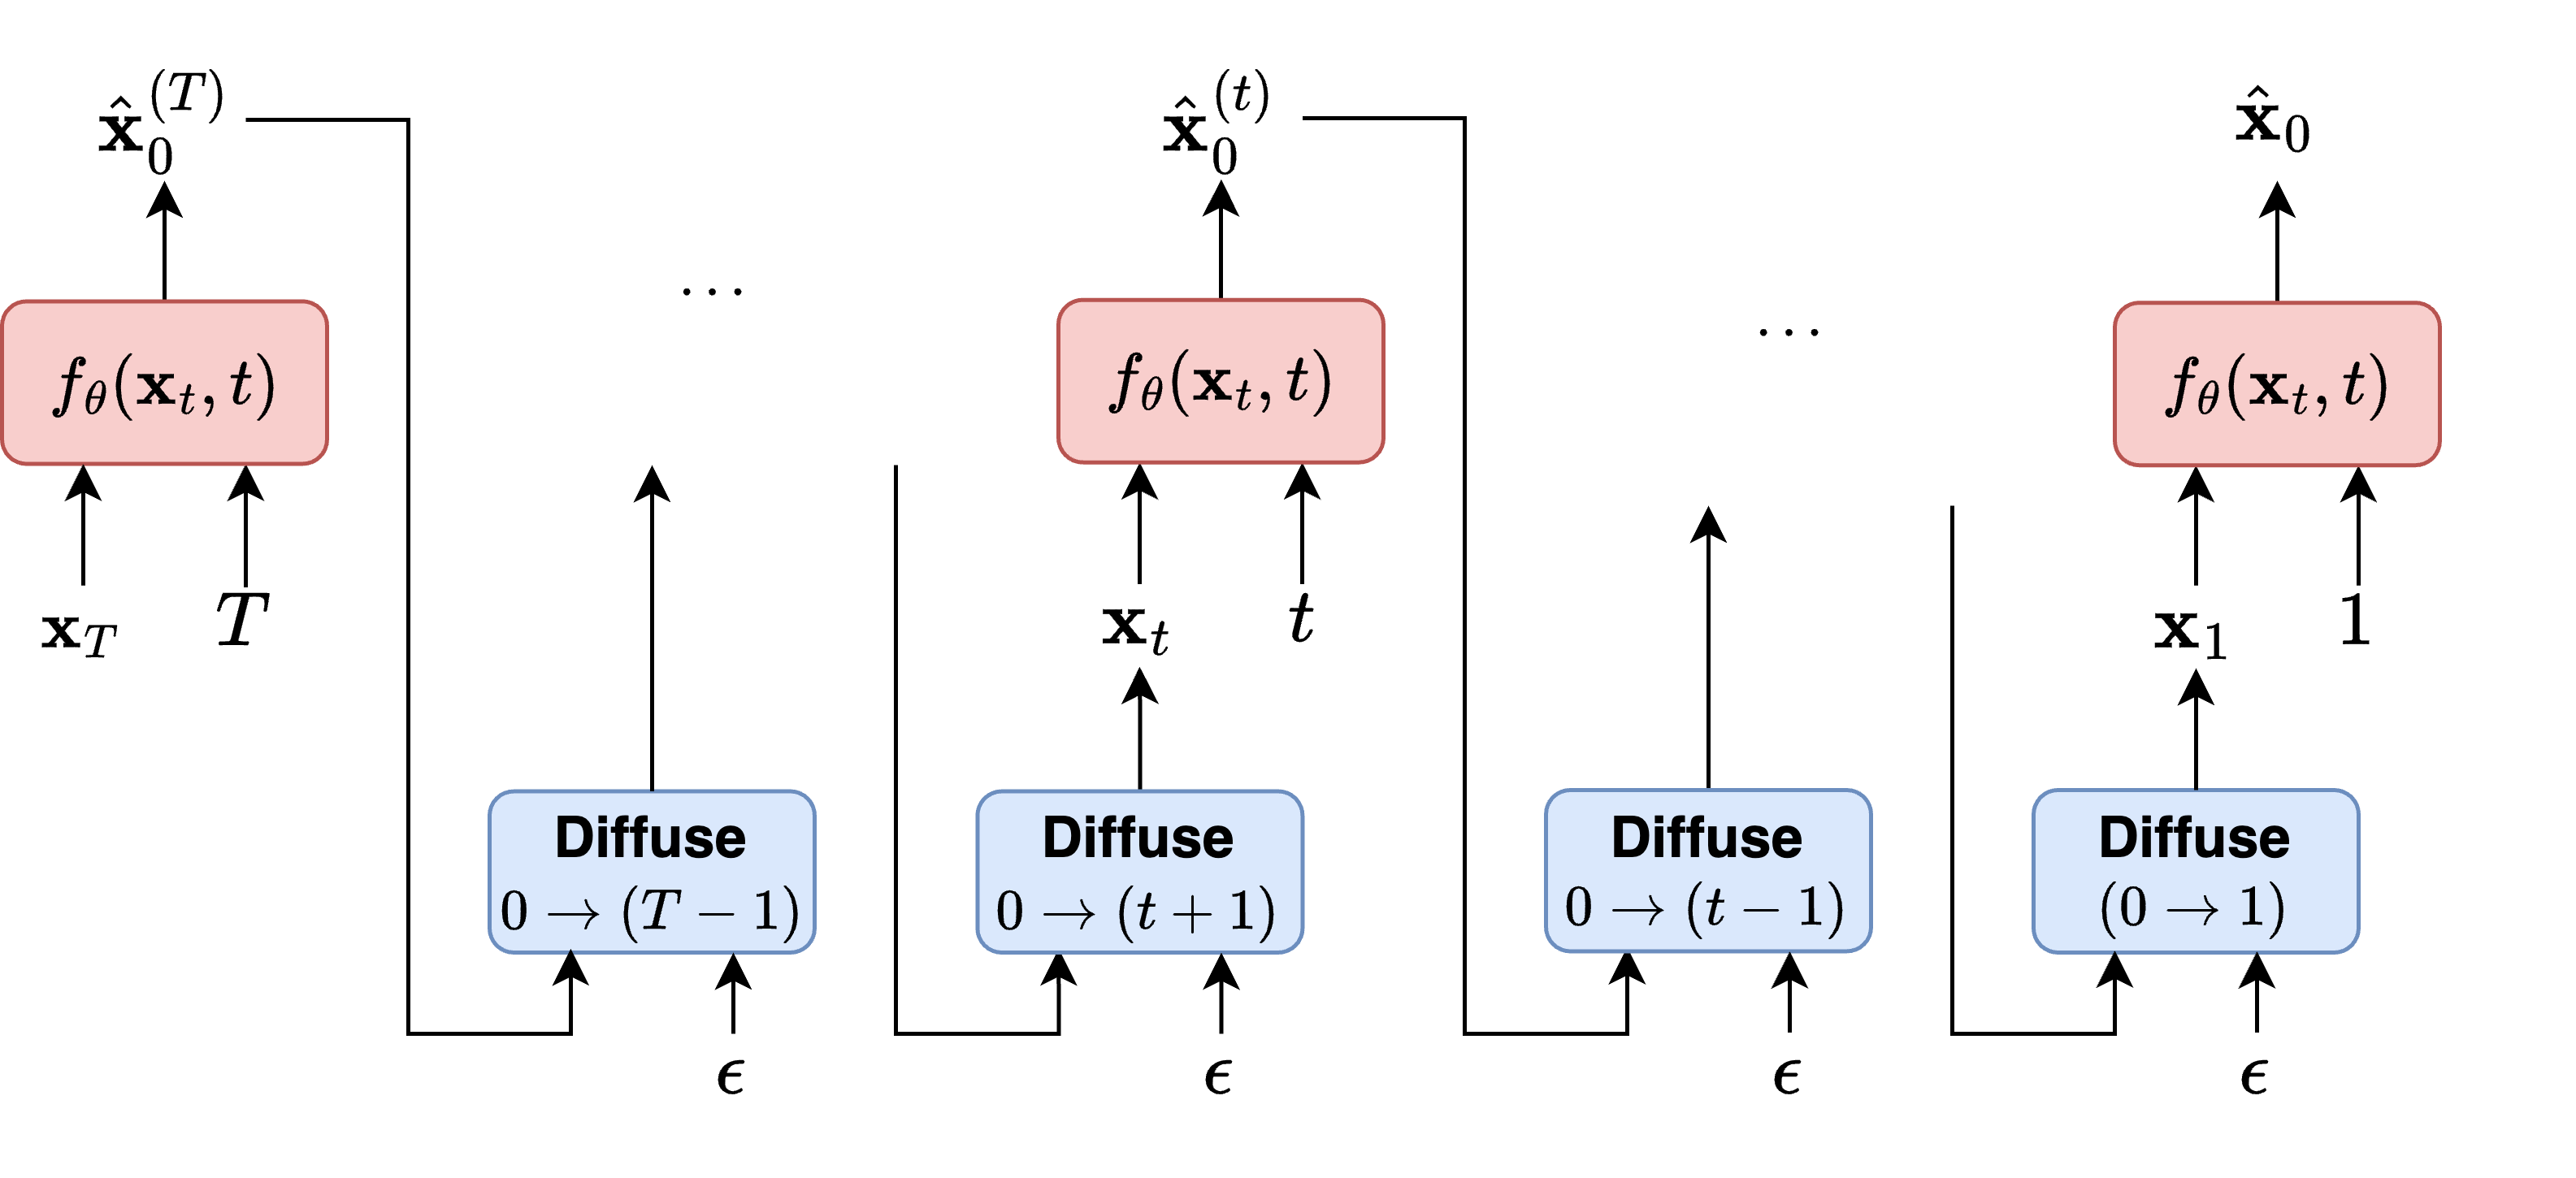
\includegraphics[width=0.95\linewidth]{SimpleX0Objective}
	\end{figure}
	
\end{frame}

\begin{frame}{So sánh $\epsilon$ objective và $\bx_0$ objective}
%$z_t = \sqrt{\bar{\alpha}_t}z_0 + \sqrt{1-\bar{\alpha}_t}\epsilon, \quad \epsilon \sim \mathcal{N}(0,I)$
%
%
%%$x_{t-1} = \sqrt{\alpha_{t-1}}\hat{x}_0 + \sqrt{1-\alpha_{t-1}}\epsilon$
%
%$\hat{z}_0 = f_\theta(z_T, t, \text{text\_embedding})$
%
%$L = \mathbb{E}_{t,z_0,\epsilon}[\|\hat{z}_0 - z_0\|_2^2]$
%
%$z_{t-1} = \sqrt{\alpha_{t-1}}\hat{z}_0 + \sqrt{1-\alpha_{t-1}}\epsilon$

\begin{figure}
	\centering
	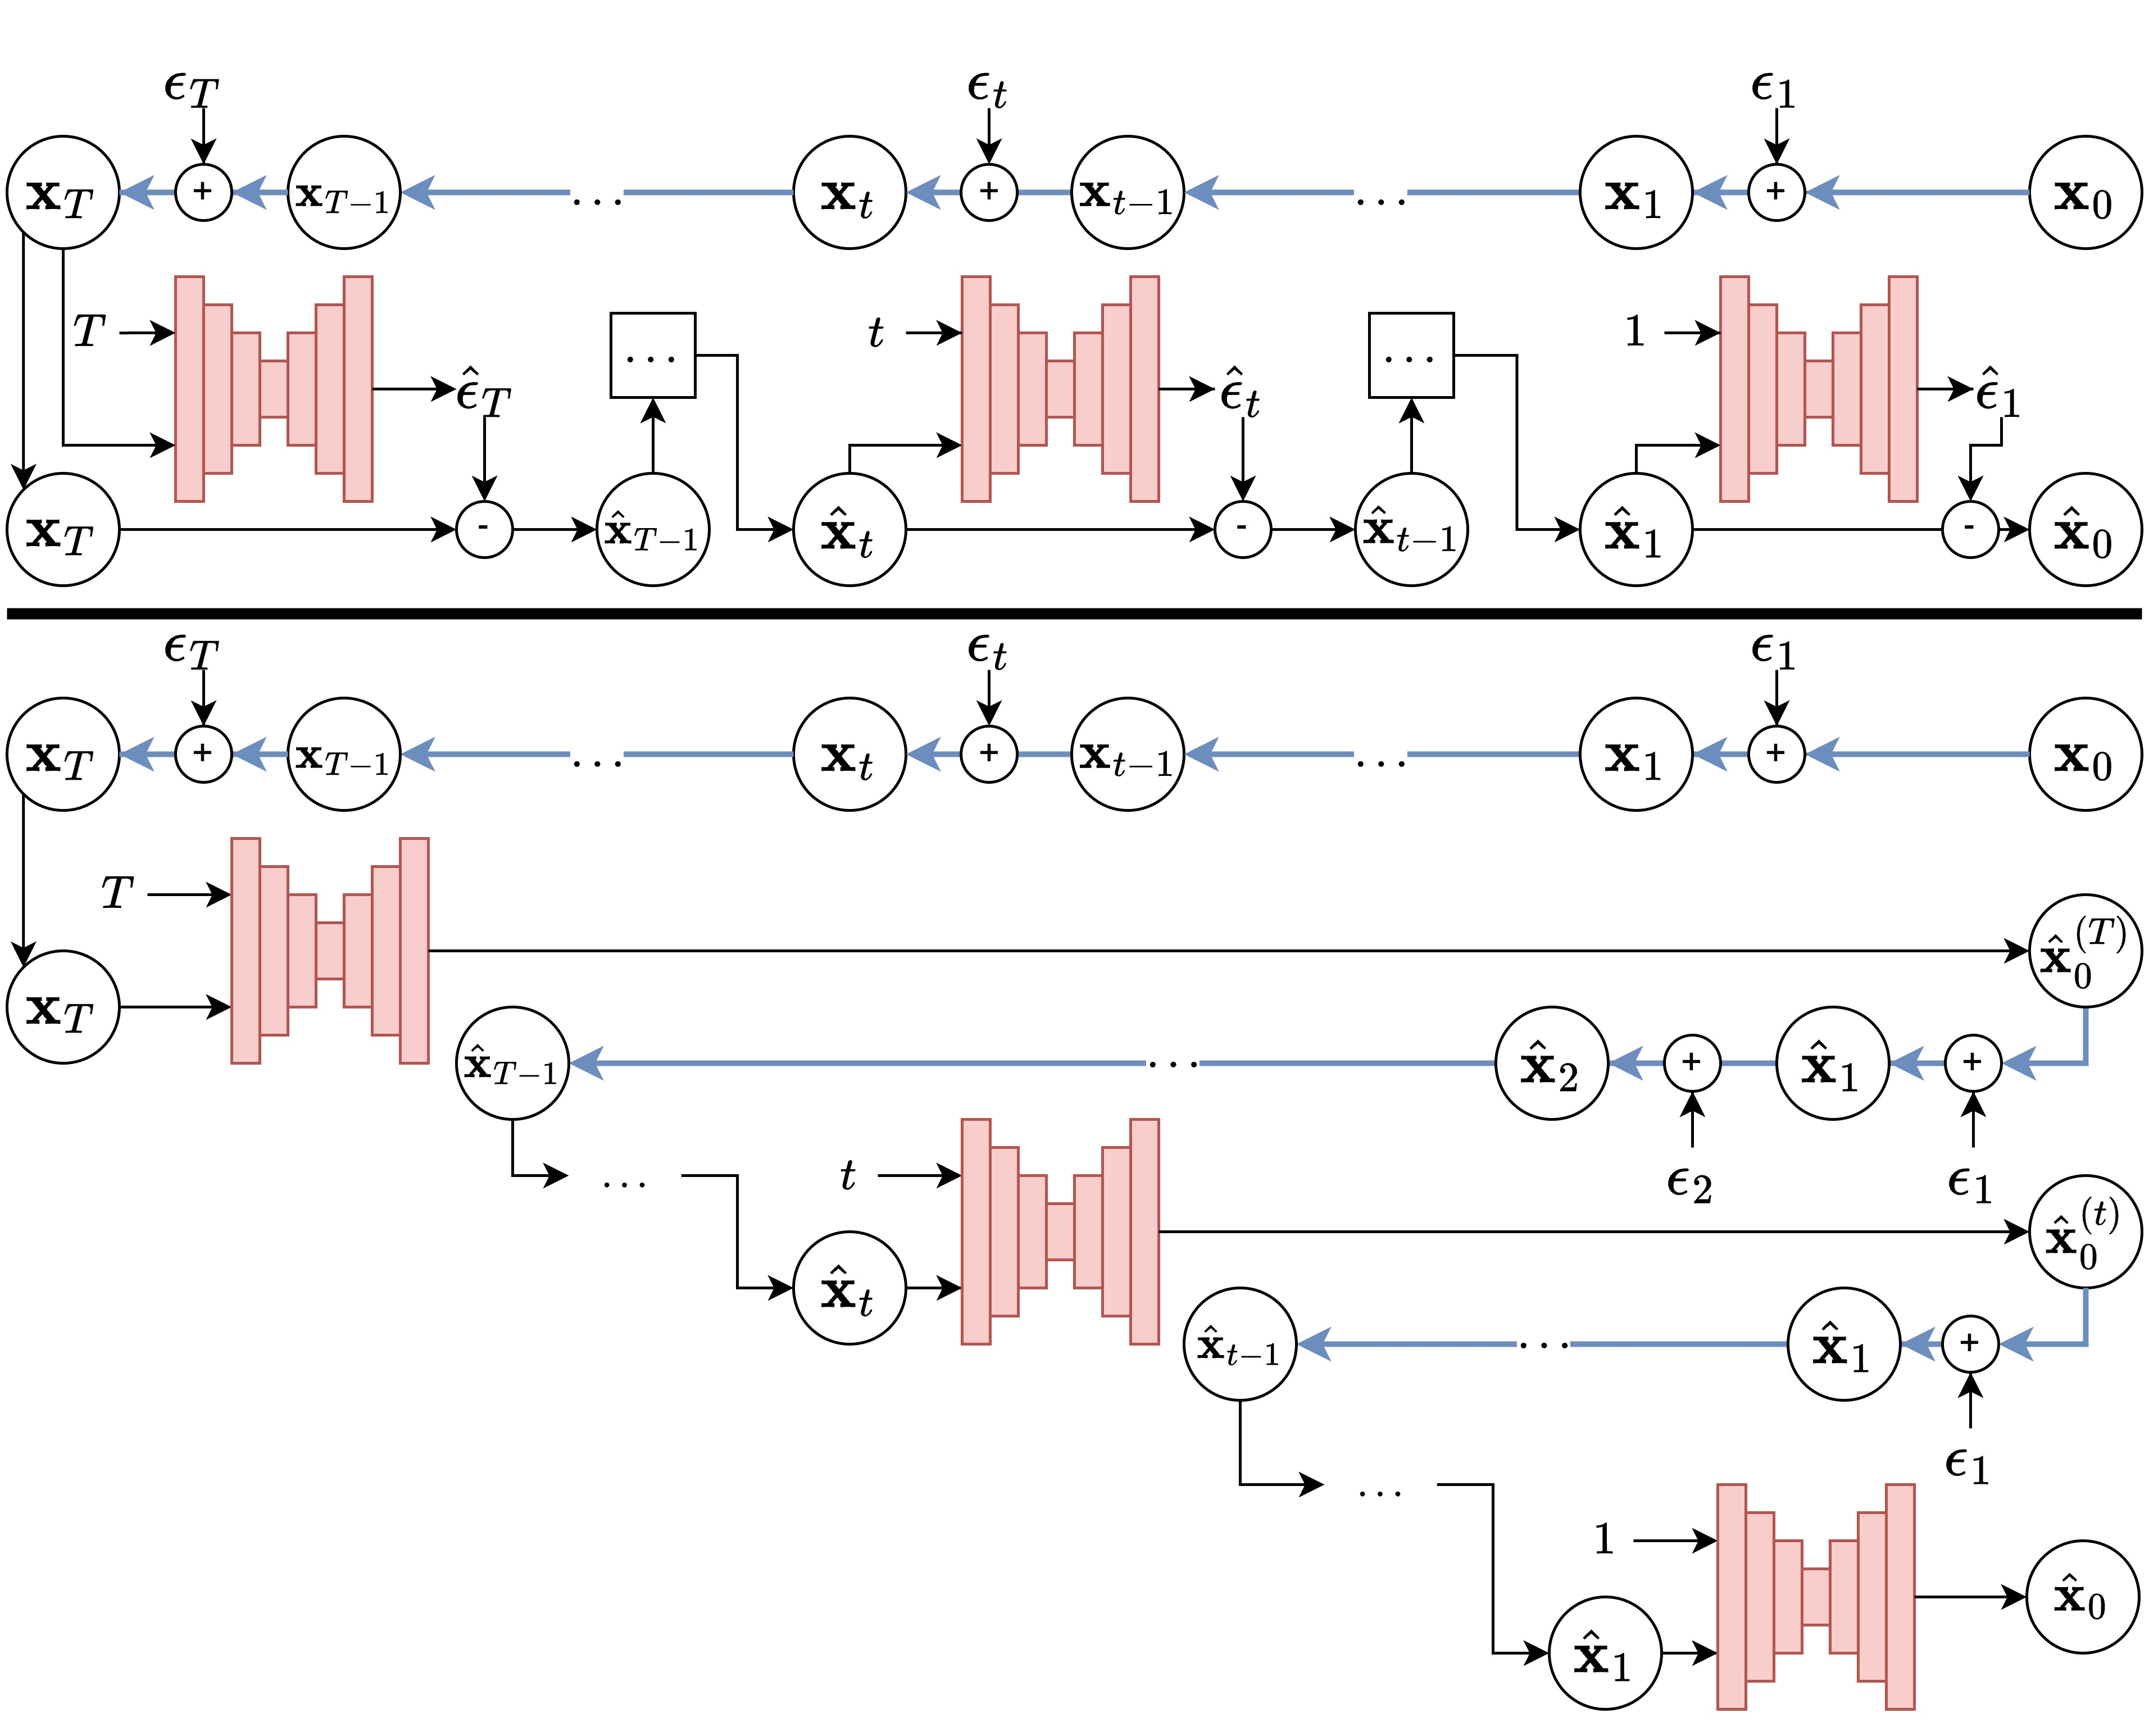
\includegraphics[width=0.95\linewidth]{X0Objective}
\end{figure}




%	
%	{Forward Process}
%	
%	\textbf{DDPM:}
%	\begin{equation}
%		q(x_t|x_{t-1}) = \mathcal{N}(x_t; \sqrt{1-\beta_t}x_{t-1}, \beta_tI)
%	\end{equation}
%	Trong đó:
%	\begin{itemize}
%		\item $\beta_t$ là lịch nhiễu (noise schedule)
%		\item $x_t$ là ảnh ở bước $t$
%		\item $\mathcal{N}$ là phân phối chuẩn (Gaussian)
%	\end{itemize}
%	
%	\textbf{DDIM:}
%	\begin{equation}
%		q(x_t|x_0) = \mathcal{N}(x_t; \sqrt{\bar{\alpha}_t}x_0, (1-\bar{\alpha}_t)I)
%	\end{equation}
%	Trong đó:
%	\begin{itemize}
%		\item $\bar{\alpha}_t = \prod_{i=1}^t(1-\beta_i)$
%		\item $x_0$ là ảnh gốc
%	\end{itemize}
%$x_t = \sqrt{\alpha_t}x_{t-1} + \sqrt{1-\alpha_t}\epsilon$

%\text{Trong đó:}
%\begin{align*}
%	& x_t: \text{là trạng thái tại thời điểm } t \\
%	& x_{t-1}: \text{là trạng thái tại thời điểm } t-1 \\
%	& \alpha_t: \text{là tham số variance scheduling } (0 < \alpha_t < 1) \\
%	& \epsilon \sim \mathcal{N}(0,1): \text{là nhiễu Gaussian}
%\end{align*}
%
%% Có thể viết dưới dạng tích lũy \bar{\alpha}
%$\text{Định nghĩa: } \bar{\alpha_t} = \prod_{i=1}^t \alpha_i$
%
%$x_t = \sqrt{\bar{\alpha_t}}x_0 + \sqrt{1-\bar{\alpha_t}}\epsilon$

%	$$\bx_{t-1} = \sqrt{\alpha_{t-1}} \left( \frac{\bx_t - \sqrt{\alpha_t} \epsilon_{\theta}(\bx_t, t)}{\sqrt{1 - \alpha_t}} \right) + \sqrt{1 - \alpha_{t-1}} \epsilon_{\theta}(\bx_t, t)$$
\end{frame}

\begin{frame}{Classifier-Free Guidance}
	\begin{columns}
		\begin{column}{0.5\textwidth}
			Để có thể học được có điều kiện (condition $c$):
%			\begin{align*}
%				\nabla p_{\gamma}(\bx_t | y) &= \nabla \log p(x_t) + \gamma \nabla p(y | \bx_t)
%			\end{align*}
%			
%			\begin{align*}
%				\nabla_{\mathbf{x}_t} \log q(\mathbf{x}_t, y)
%				&= \nabla_{\mathbf{x}_t} \log q(\mathbf{x}_t) + \nabla_{\mathbf{x}_t} \log q(y \vert \mathbf{x}_t)		
%			\end{align*}
			
		\end{column}
		
		\begin{column}{0.5\textwidth}
			\begin{figure}
				\centering
				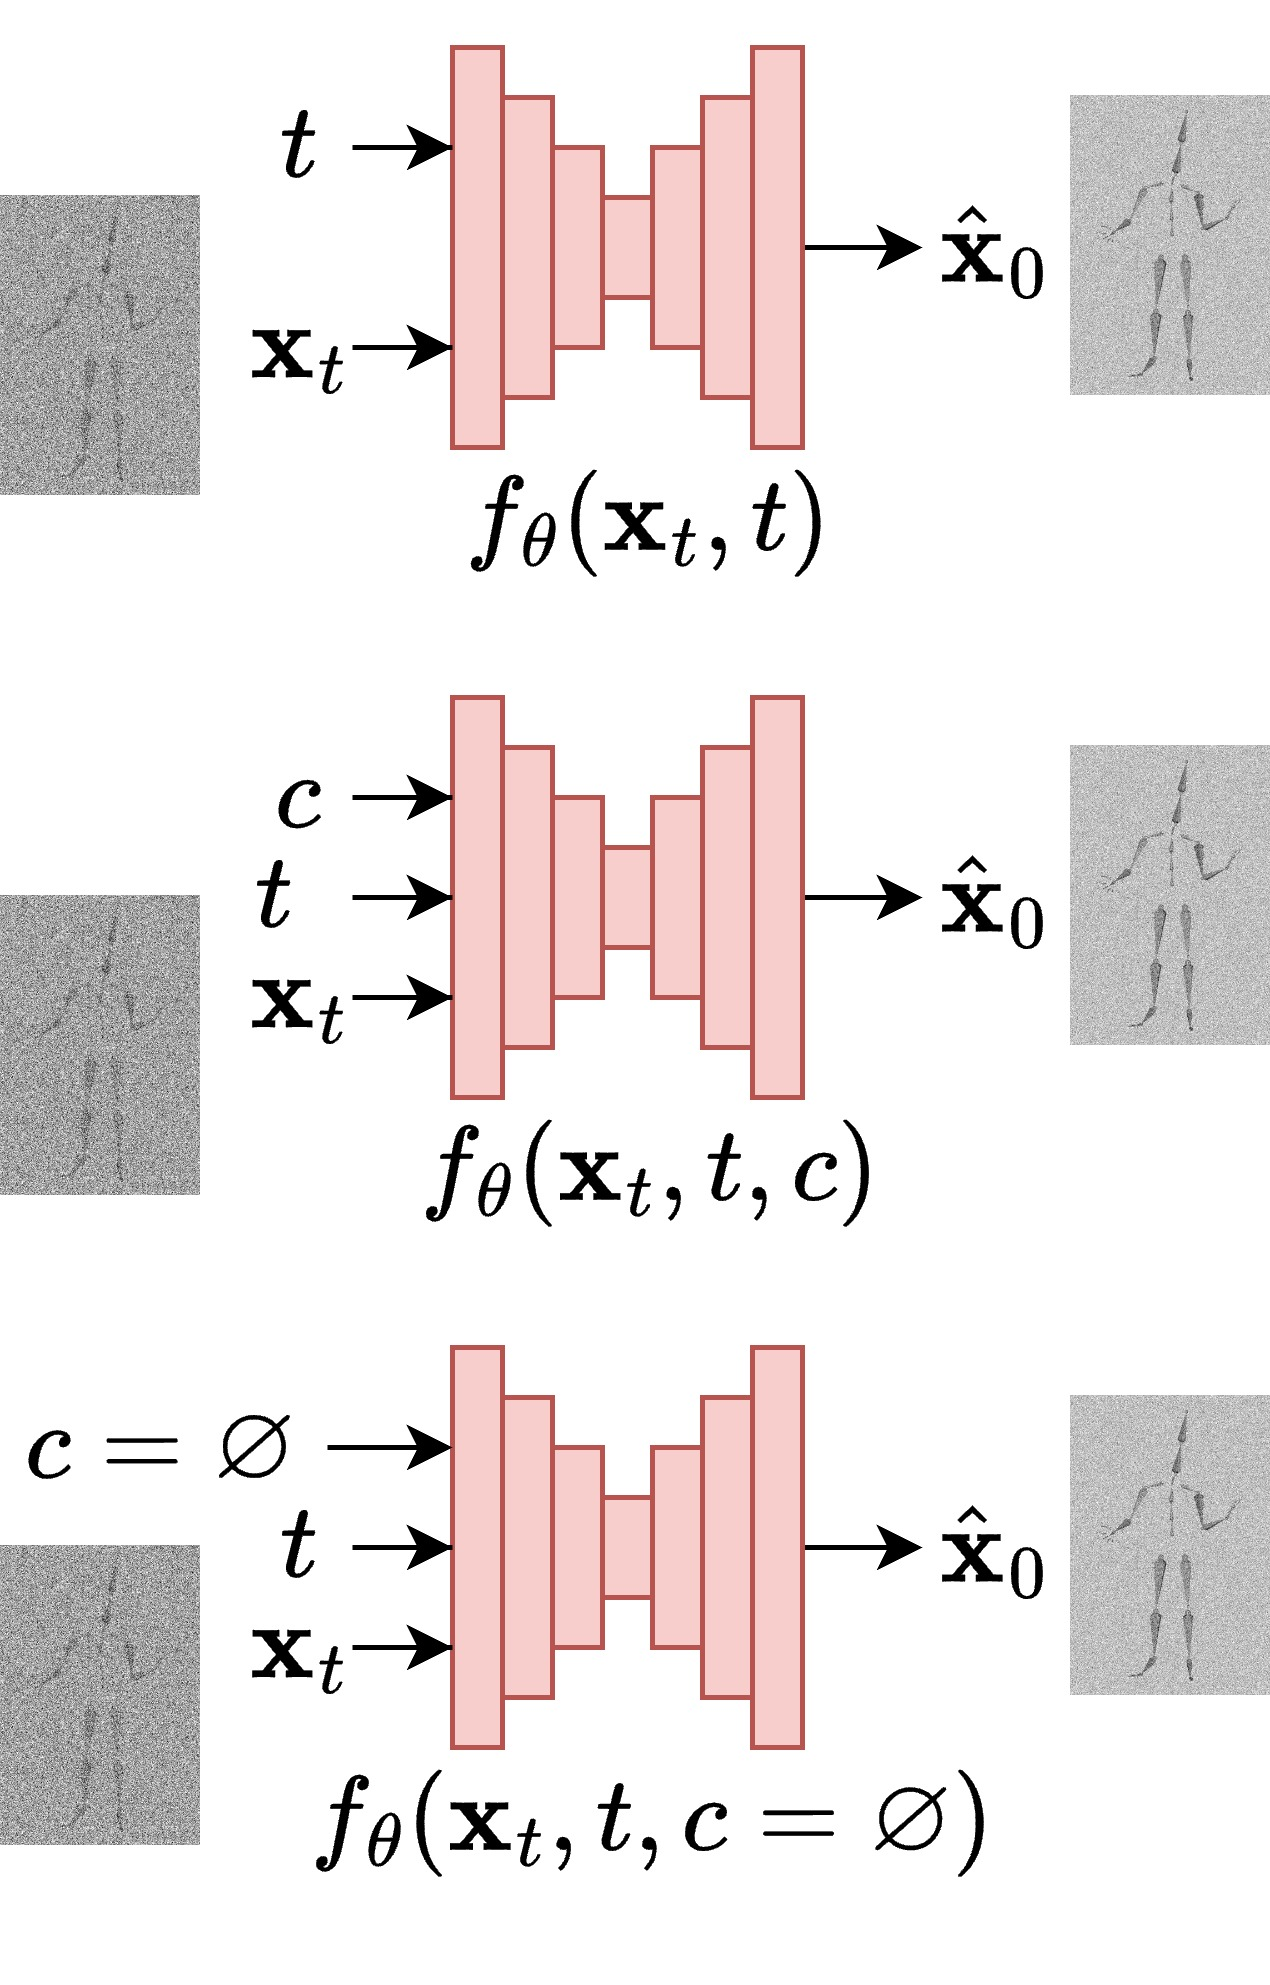
\includegraphics[width=0.95\linewidth]{ConditionDiffusion}
			\end{figure}
		\end{column}
	\end{columns}
	

	
\end{frame}


\begin{frame}{Condition Diffusion với $\mathbf{x}_0$ Objective}
	\begin{figure}
		\centering
		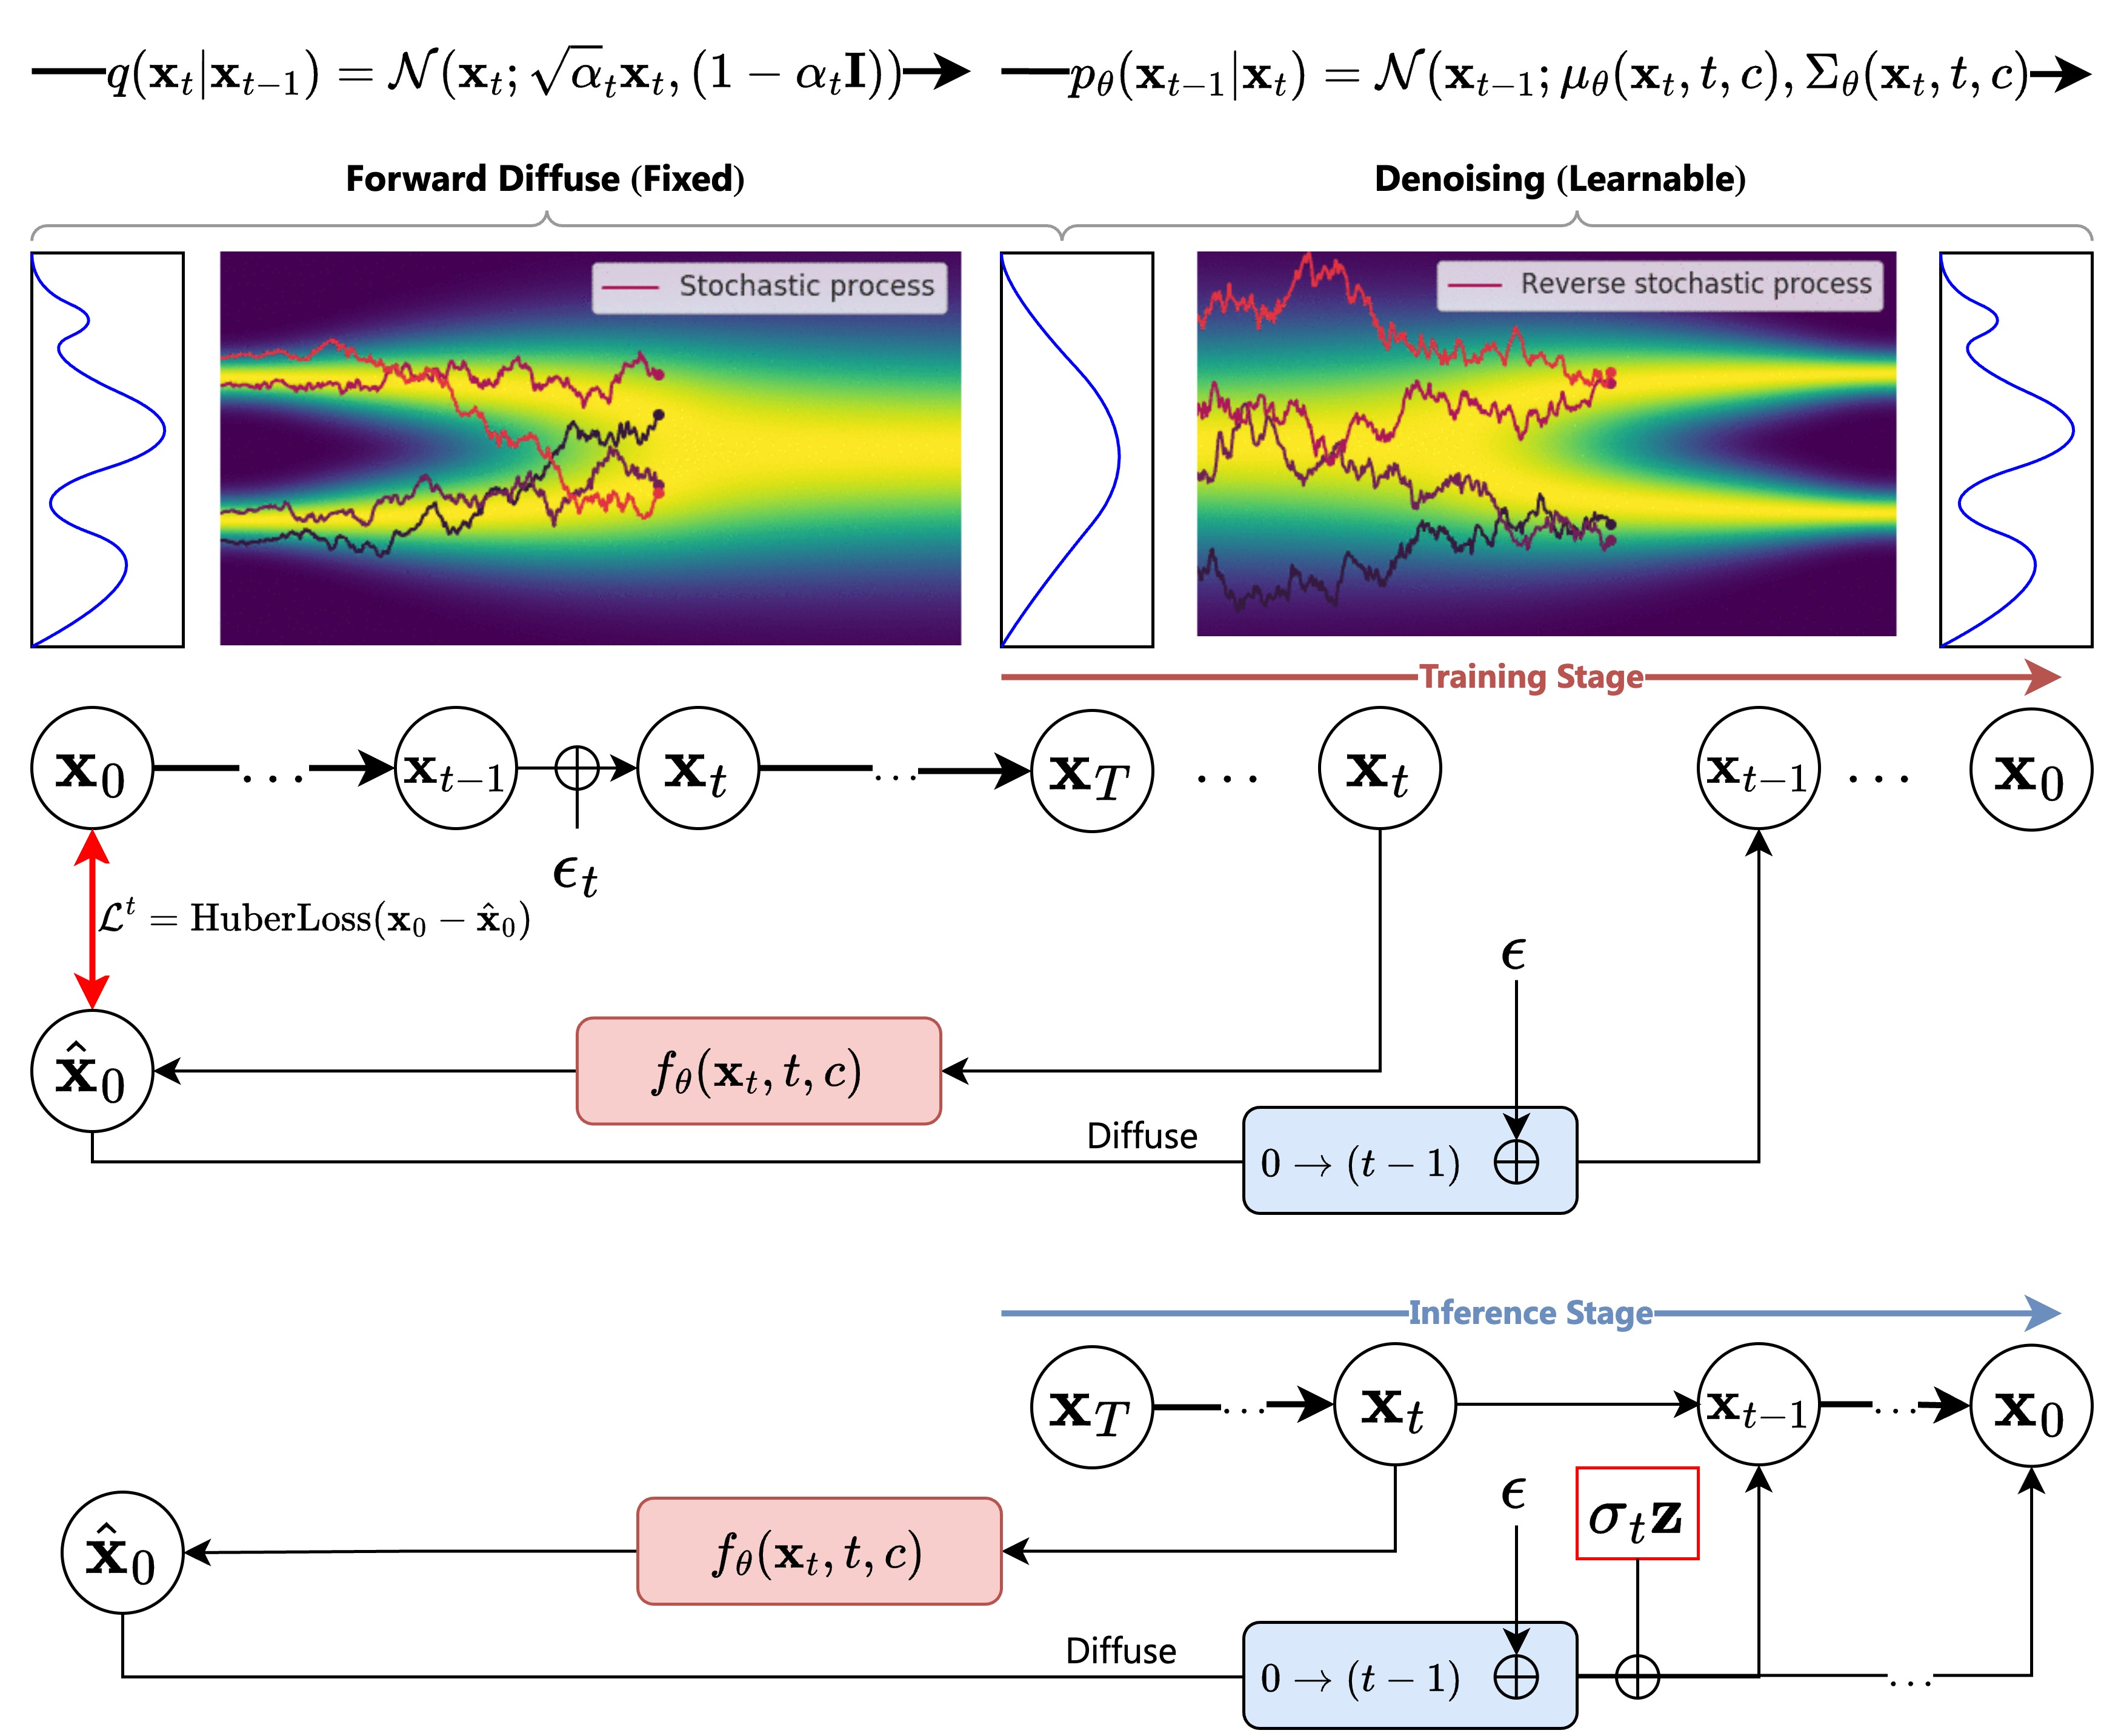
\includegraphics[width=0.95\linewidth]{TrainingAndSampling.jpg}
	\end{figure}
\end{frame}




\begin{frame}{Forward Diffusion Process}
%	 & \text{ ;where } \boldsymbol{\epsilon}_{t-1}, \boldsymbol{\epsilon}_{t-2}, \dots \sim \mathcal{N}(\mathbf{0}, \mathbf{I})
\small
\begin{itemize}[]
	\item Đặt $\alpha_t = 1 - \beta_t$, $\bar{\alpha}_t = \prod_{i=1}^t \alpha_i$
\end{itemize}
\vspace{-15pt}
\begin{align*}
	\mathbf{x}_t & = \sqrt{\alpha_t}\mathbf{x}_{t-1} + \sqrt{1 - \alpha_t} \boldsymbol{\epsilon}_{t-1} \\
						& = \sqrt{\alpha_t \alpha_{t-1}} \mathbf{x}_{t-2} + \sqrt{1 - \alpha_t \alpha_{t-1}} \bar{\boldsymbol{\epsilon}}_{t-2} \\
						& = \dots \\
						& = \sqrt{\bar{\alpha}_t}\mathbf{x}_0 + \sqrt{1 - \bar{\alpha}_t}\boldsymbol{\epsilon} \\
						q(\mathbf{x}_t \vert \mathbf{x}_{t-1}) &= \mathcal{N}(\mathbf{x}_t; \sqrt{\alpha_t} \mathbf{x}_{t-1}, (1 - \alpha_t)\mathbf{I}) \\ 
						\rightarrow q(\mathbf{x}_t \vert \mathbf{x}_0) &= \mathcal{N}(\mathbf{x}_t; \sqrt{\bar{\alpha}_t} \mathbf{x}_0, (1 - \bar{\alpha}_t)\mathbf{I})
\end{align*}
\vspace{-20pt}
%\begin{figure*}
	
%	& \text{ ;where } \bar{\boldsymbol{\epsilon}}_{t-2} \text{ merges two Gaussians (*).} \\
\begin{columns}
\begin{column}{0.5\textwidth}
	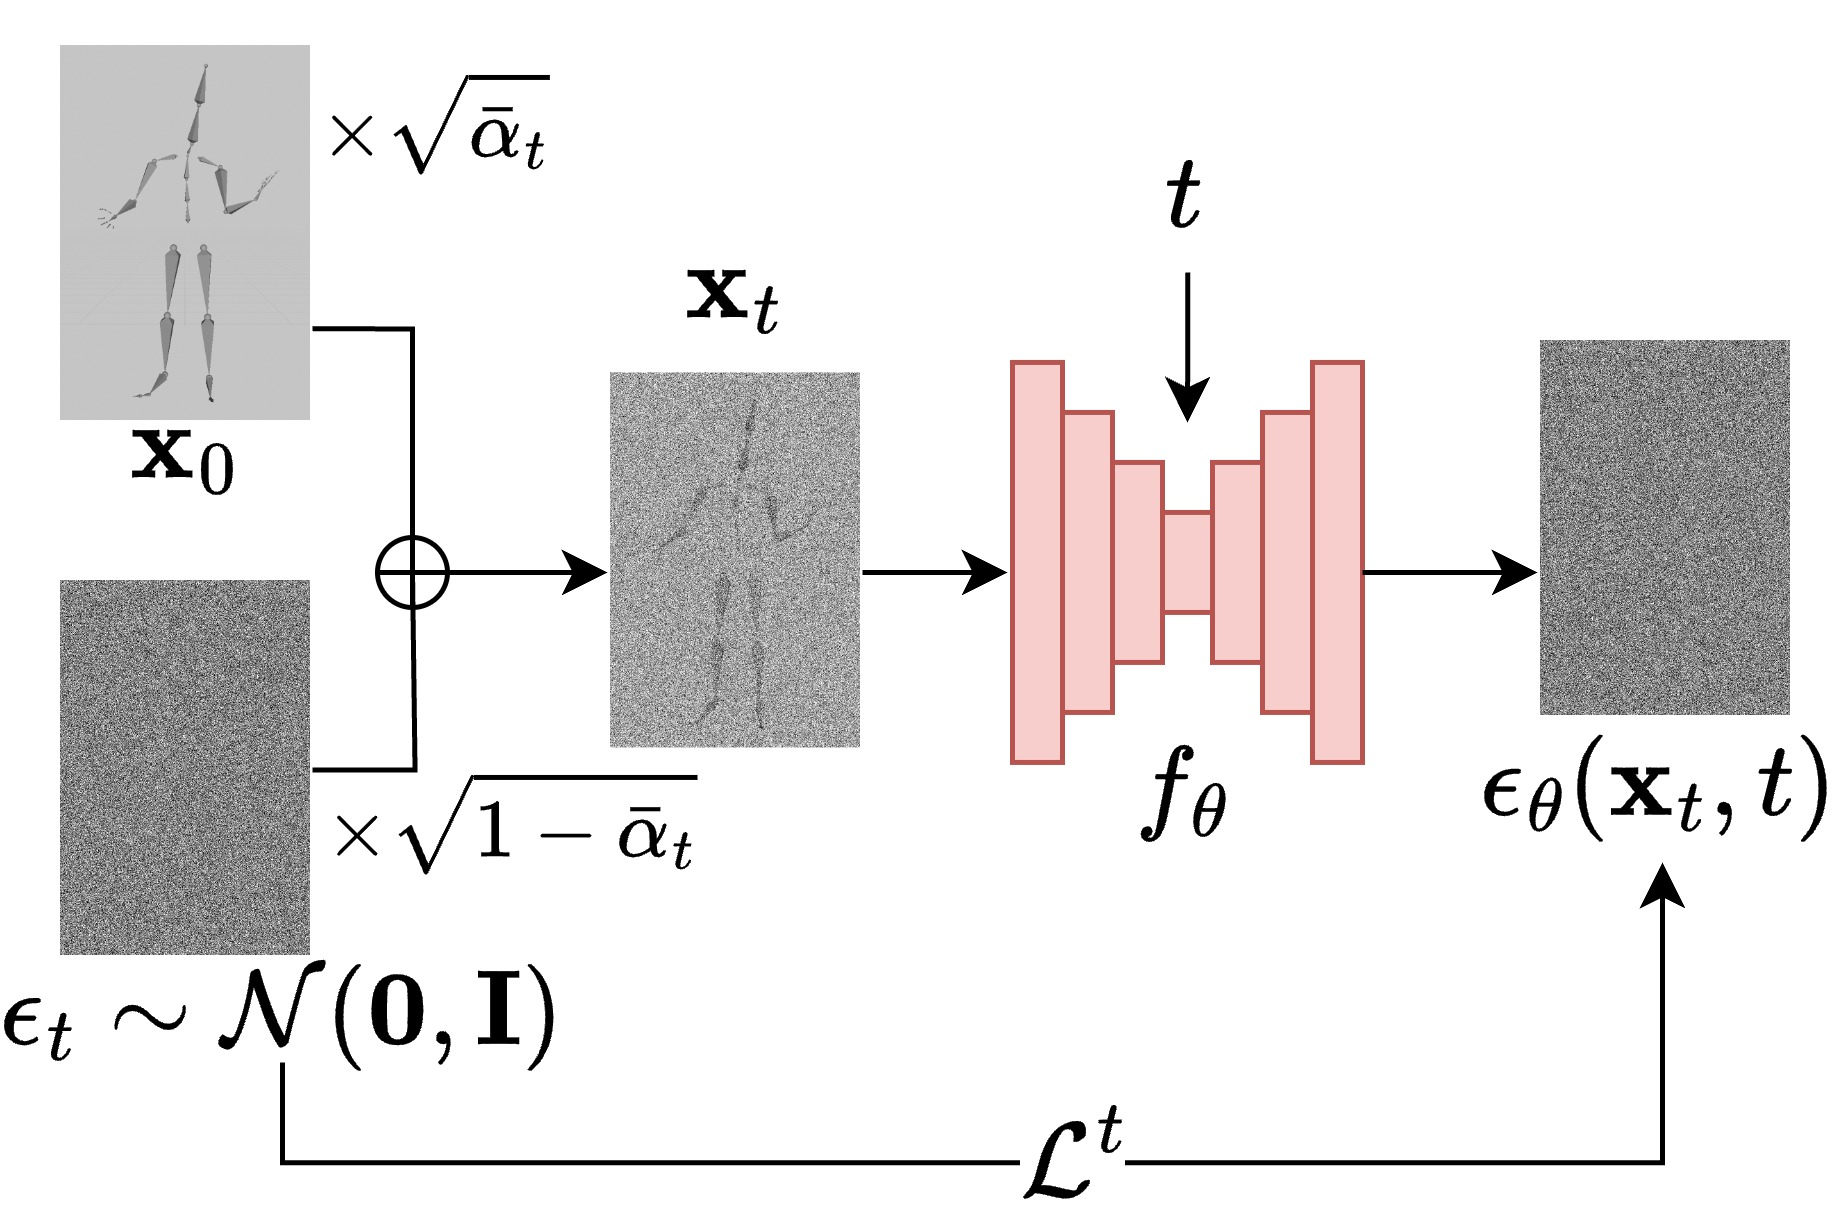
\includegraphics[width=\textwidth]{AlgorithmForwardDiffusion.png}
\end{column}


	
\begin{column}{0.5\textwidth}
	\footnotesize
	\begin{algorithm}[H]
		\caption{Training} \label{alg:training}
		\begin{algorithmic}[1]
			\footnotesize
			\Repeat
			\State $\bx_0 \sim q(\bx_0)$
			\State $t \sim \mathrm{Uniform}(\{1, \dotsc, T\})$
			\State $\bepsilon\sim\mathcal{N}(\bzero,\bI)$
			\State Take gradient descent step on
			\Statex $\qquad \grad_\theta \left\| \bepsilon - \bepsilon_\theta(\mathbf{x}_t, t) \right\|^2$
			\Until{converged}
		\end{algorithmic}
	\end{algorithm}
\end{column}
\end{columns}
\end{frame}

\begin{frame}{Reverse Diffusion Process}
	
\small
$p_{\theta}(\mathbf{x}_T) = \mathcal{N} (0, \mathbf{I}) \qquad 
p_{\theta}(\mathbf{x}_{t-1} | \mathbf{x}_t) = \mathcal{N}(\mathbf{x}_t; \mu_\theta(\mathbf{x}_t), \sigma_t^2 \mathbf{z})
$
%\begin{columns}
%	\begin{column}{0.5\textwidth}
%		
%	\end{column}
%	\begin{column}{0.5\textwidth}
%		
%	\end{column}
%\end{columns}

$\mu_\theta(\mathbf{x}_t) = 
\frac{1}{\sqrt{\alpha_{t}}} ( \mathbf{x}_t - 
\frac{1-\alpha_t}{ \sqrt{1 - \bar{\alpha_{t}} }}
\epsilon_{\theta} (\mathbf{x}_t,t))$
%\vspace{-20pt}
%\begin{figure*}

%	& \text{ ;where } \bar{\boldsymbol{\epsilon}}_{t-2} \text{ merges two Gaussians (*).} 

\begin{columns}
	\begin{column}{0.43\textwidth}
		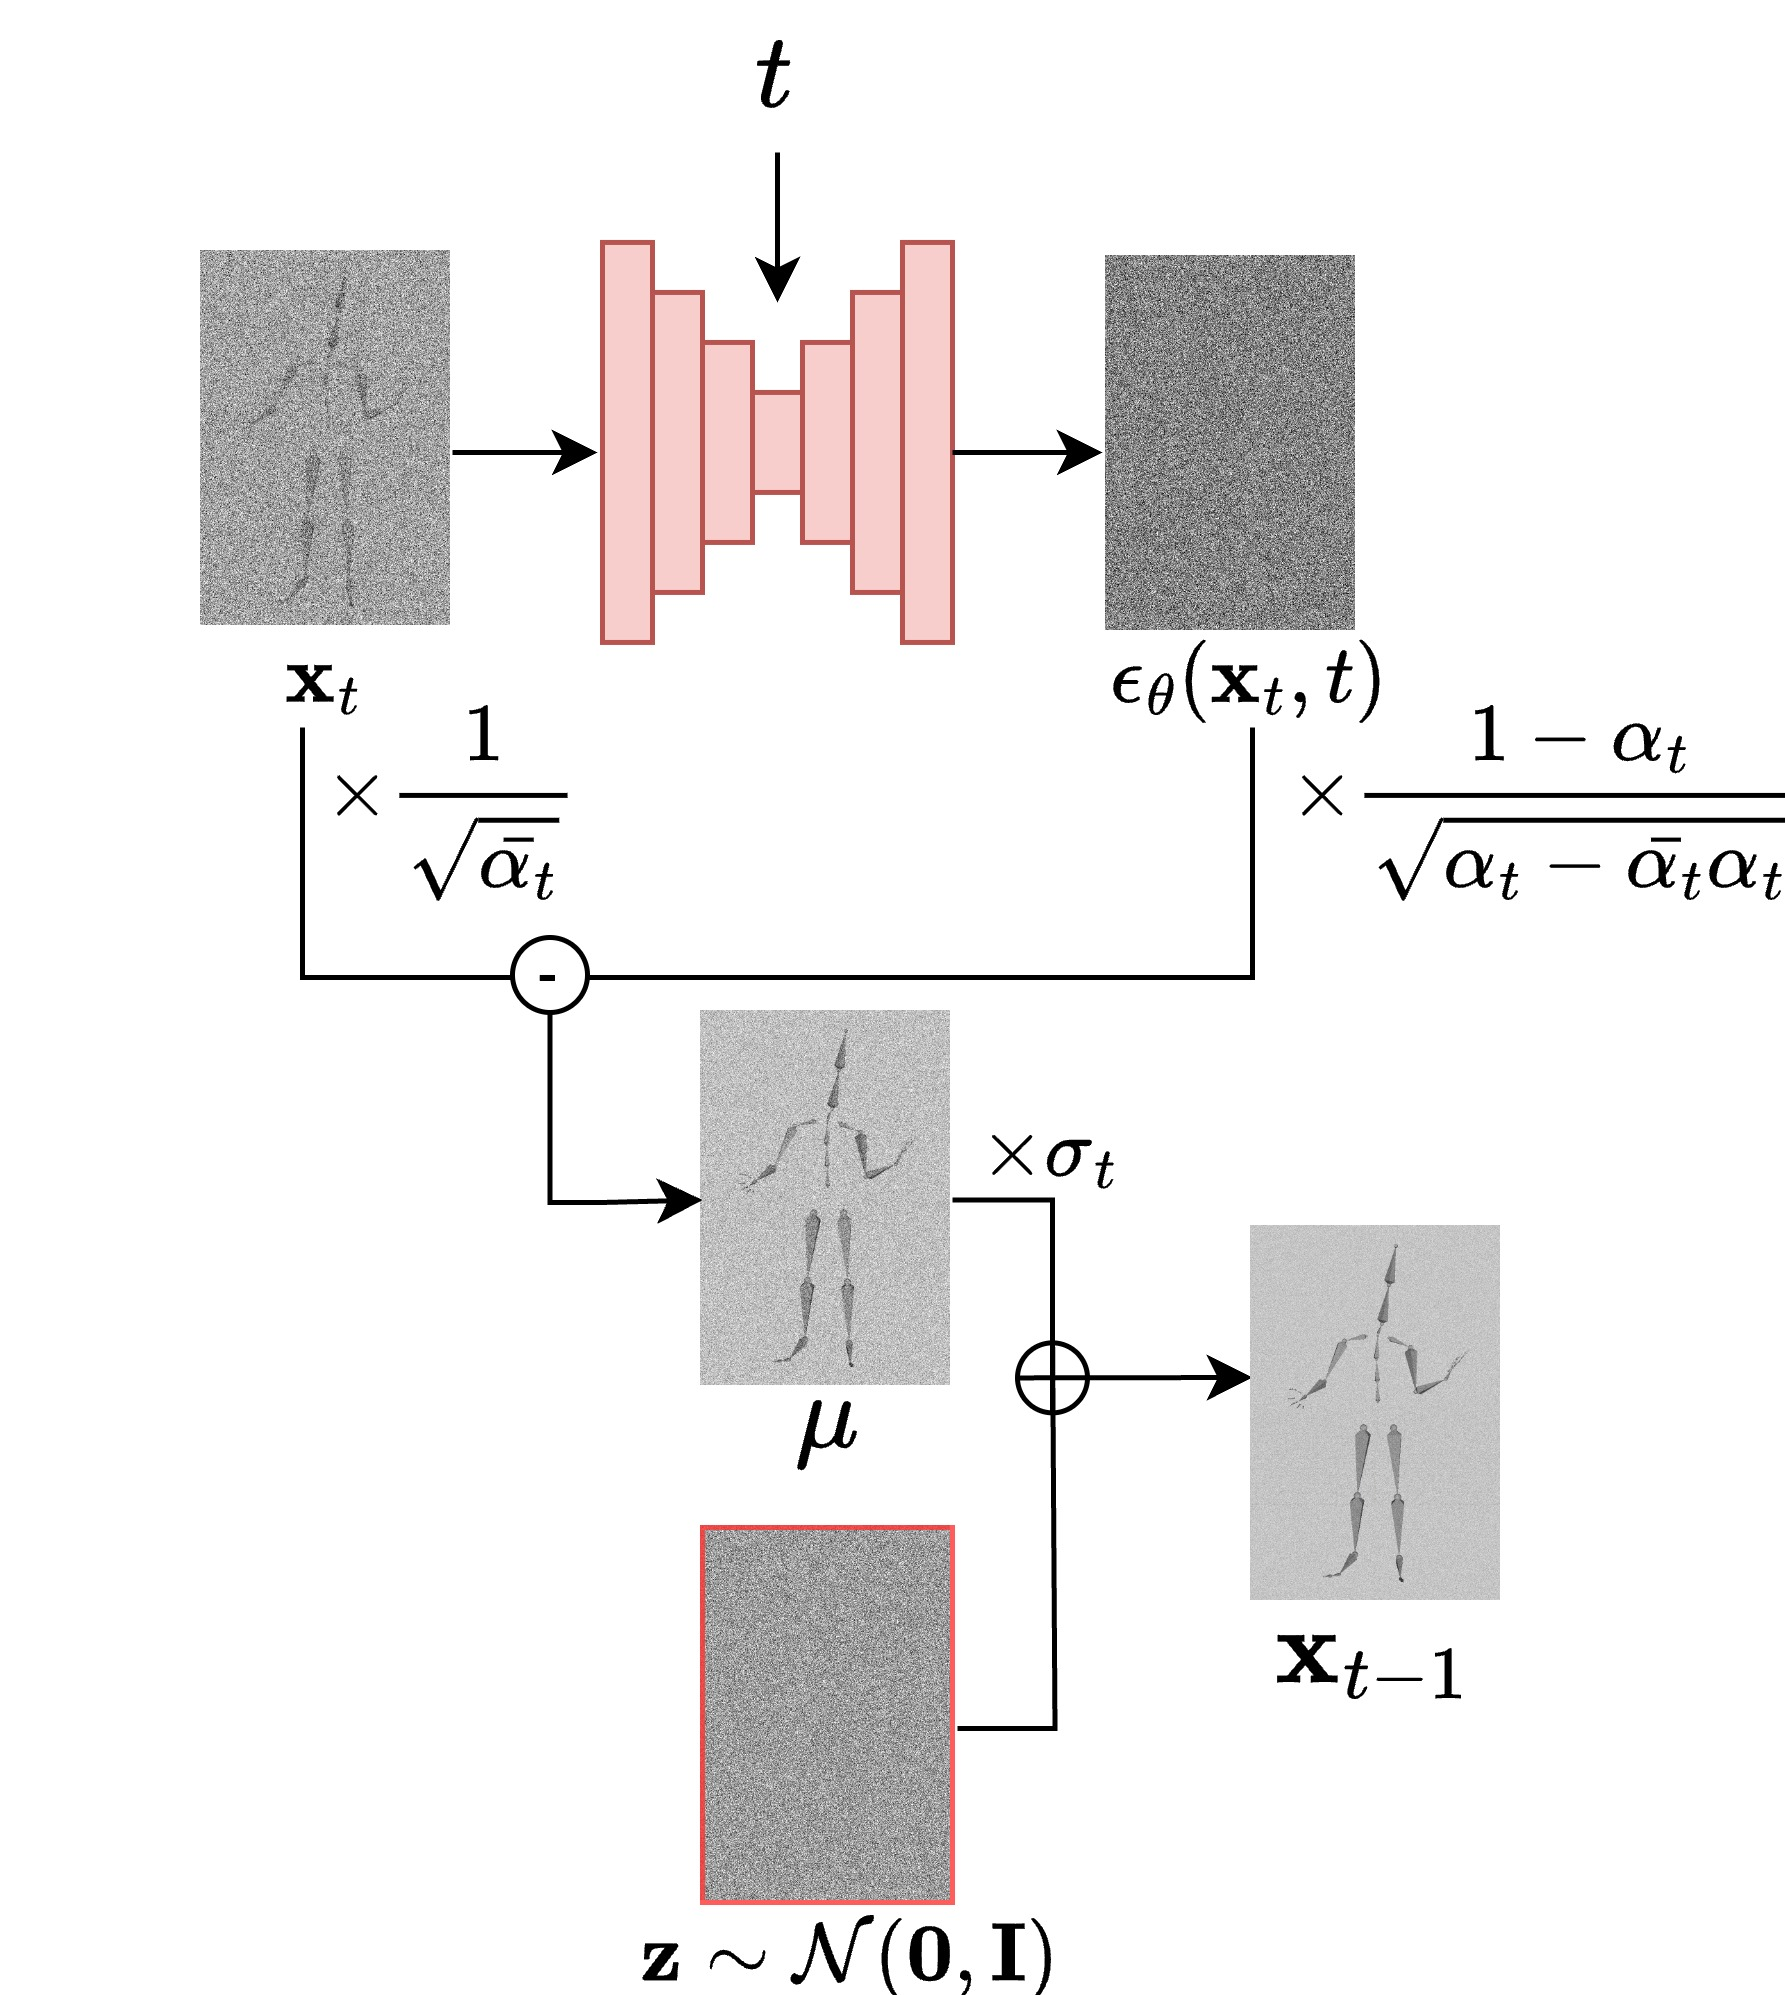
\includegraphics[width=\textwidth]{AlgorithmSamplingDiffusion.png}
	\end{column}
	
	\begin{column}{0.57\textwidth}
		\footnotesize
		\begin{algorithm}[H]
			\caption{Sampling} \label{alg:sampling}
			\footnotesize
			\begin{algorithmic}[1]
					\footnotesize
					\State $\bx_T \sim \mathcal{N}(\bzero, \bI)$
					\For{$t=T, \dotsc, 1$}
					\State $\bz \sim \mathcal{N}(\bzero, \bI)$ if $t > 1$, else $\bz = \bzero$
					\State $\mu = \frac{1}{\sqrt{\alpha_t}}\left( \bx_t - \frac{1-\alpha_t}{\sqrt{1-\bar\alpha_t}} \bepsilon_\theta(\bx_t, t) \right) $
					\State $\bx_{t-1} = \mu + \sigma_t \bz$
%					+ \sigma_t \bz
%_\theta (\mathbf{x}_t,	 t)
					\EndFor
					\State \textbf{return} $\bx_0$
					\vspace{.04in}
				\end{algorithmic}
		\end{algorithm}
\end{column}

\end{columns}

\end{frame}

%	\algrenewcommand\algorithmicindent{0.5em}
%	\begin{figure}[t]
	%		\begin{minipage}[t]{0.495\textwidth}
		%			\begin{algorithm}[H]
			%				\caption{Training} \label{alg:training}
			%				\small
			%				\begin{algorithmic}[1]
				%					\Repeat
				%					\State $\bx_0 \sim q(\bx_0)$
				%					\State $t \sim \mathrm{Uniform}(\{1, \dotsc, T\})$
				%					\State $\bepsilon\sim\mathcal{N}(\bzero,\bI)$
				%					\State Take gradient descent step on
				%				\Statex $\qquad \grad_\theta \left\| \bepsilon - \bepsilon_\theta(\sqrt{\bar\alpha_t} \bx_0 + \sqrt{1-\bar\alpha_t}\bepsilon, t) \right\|^2$
				%					\Until{converged}
				%				\end{algorithmic}
			%			\end{algorithm}
		%		\end{minipage}
	%		\begin{minipage}[t]{0.495\textwidth}
		%			
		%		\end{minipage}
	%		\vspace{-1em}
	%	\end{figure}




	
%	
%		if $L$ is not known (usually the case), can use the following line search:
%	\noindent\rule[-5pt]{\textwidth}{0.4pt}
%	
%	\noindent\rule[10pt]{\textwidth}{0.4pt}
%	
%	typical value of $\beta$ is $1/2$, and 
%	\[
%	\hat{f}_\lambda(x,y) = f(y) + \nabla f(y)^T (x - y) + 
%	(1/2\lambda)\|x - y\|_2^2
%	\]